\documentclass[11pt,twoside]{memoireuqam1.3}
\usepackage{amssymb,graphicx,stackengine,xcolor}
\def\ucr{\scalebox{1}{\stackinset{c}{}{c}{-.2pt}{%
			  \textcolor{white}{\sffamily\bfseries\small ?}}{%
				    \rotatebox{45}{$\blacksquare$}}}}
\uqammemoire   %% Pour la page titre d'un mémoire

\usepackage{graphicx}% Pour les figures
%\usepackage[T1]{fontenc} % pour windows surtout, pas bon
%\usepackage[utf8x]{inputenc} % Pour utiliser les caractères accentués sous Unix
\usepackage{longtable}
\usepackage{booktabs}
\usepackage[french]{babel}
\usepackage{xltxtra}
\usepackage{fancyvrb}
\usepackage{float}
\usepackage{alltt}
\usepackage{url}
\usepackage{tabularx}
%\usepackage[usenames]{color}
\usepackage{fnamed}
%\usepackage{lmodern}
%\usepackage[cyr]{aeguill} % old school, dépassé
%\usepackage[font=small]{caption}
\usepackage{afterpage}

\newcommand\blankpage{%
	\null
	\thispagestyle{empty}%
	\addtocounter{page}{-1}%
\newpage}

%\input macros  % Pour les définitions personnelles

\floatstyle{plain}
\restylefloat{figure}

\begin{document}

%%%%%%%%%%%%%%%%%%%%
% Pour la page titre
%%%%%%%%%%%%%%%%%%%%

% Le titre ne supporte pas les accent simples
\title{Des cha\^ines de caract\`eres efficaces et r\'esistantes au passage \`a l'\'echelle, une proposition de mod\'elisation pour les langages de programmation \`a objets}
\author{Lucas Bajolet}
\degreemonth{Juin}
\degreeyear{2016}
\uqammemoire
% ou
% \uqamthese   %% Pour la page titre d'une thèse
% ou
% \uqamrapport %% Pour la page titre d'un rapport

% Le département doit être modifié dans memoireuqam1.3.cls

\thispagestyle{empty}        % La page titre n'est pas numérotée
\maketitle

%%%%%%%%%%%%%%%%%%%%
% Page préliminaires
%%%%%%%%%%%%%%%%%%%%
%\renewcommand \bibname{R\'EF\'ERENCES}% FACULTATIF
%Enlever le commentaire, si vous voulez qu'apparaisse le titre RÉFÉRENCES
% plutôt que BIBLIOGRAPHIE

\renewcommand \listfigurename{LISTE DES FIGURES}
\renewcommand \appendixname{APPENDICE}
\renewcommand \figurename{Figure}
\renewcommand \tablename{Tableau}

\pagenumbering{roman} % numérotation des pages en chiffres romains
\addtocounter{page}{1} % Pour que les remerciements commencent à la page ii
\cleardoublepage
\thispagestyle{empty} % pas numérotée
   \parskip=0pt
   \vspace*{0.1 truecm} 
   \begin{center}
    {\uppercase { REMERCIEMENTS }}\par
   \end{center}
   \nobreak \vspace*{1.10 truecm}
   \parskip=2ex

Je tiens à remercier tous les gens avec qui j'ai pu travailler ces dernières années, particulièrement Jean Privat, mon directeur de recherche, pour les cafés pris dans son bureau entrecoupés de discussions constructives et les enseignements qu'il m'a transmis.
Alexis et Alexandre, mes aînés au sein du Grésil, Romain (dont certains diront qu'il n'est plus stagiaire), Philippe, Fred (qui dit-on s'est transformé en plante), et l'ensemble des stagiaires qui sont venus travailler sur le projet Nit et leur patience face a mon syndrôme des jambes sans repos coordonnées a la musique (brutale, certains diront) que j'écoutais sans arrêt durant les trois années qu'ont duré mon travail.
Je remercie également mes amis, Mathieu, Alex, Geoffrey/Romain, les colocs qui ont contribué à ralentir mon travail à renfort de bières, ma foi délicieuses, et de journées oisives à regarder des films, mais sans qui la vie aurait été bien ennuyeuse; Florent, Marion, Nico, Anthony, Peggy, JP, Ariane, Arabelle, etc., qui n'ont pas manqué de me demander régulièrement comment mon mémoire avançait, qui ont toujours pris avec humour ma sempiternelle réponse "Ça recule pas!", et qui vont perdre leur éternel ami étudiant à la remise de ce papier.
Merci également à Louise Laforest, professeur et directrice du Département d'informatique ainsi qu'a son personnel, Kathleen, Mylène, Marie-Claude, pour les grands moments passés lors du maintenant traditionnel "Jeudi apporte ton lunch" et la quantité incroyable de sucreries apportées à chaque semaine; mon médecin n'est pas content, mais il n'y a toujours pas de traces de diabètes dans mon bilan sanguin il semblerait !
Merci {\fontspec{DejaVu Sans}�}galement {\fontspec{DejaVu Sans}�} UTF-8 pour sa coop{\fontspec{DejaVu Sans}�}ration {\fontspec{DejaVu Sans}�} l'{\fontspec{DejaVu Sans}�}criture de ce m{\fontspec{DejaVu Sans}�}moire.
Finalement, je remercie ma famille, et plus particulièrement mes parents, pour m'avoir encouragé à venir au Québec pour poursuivre mes études, et qui m'ont soutenu tout au long de ma vie.

\tableofcontents % Pour générer la table des matières
\listoffigures % Pour générer la liste des figures
\listoftables % Pour générer la liste des tableaux
\begin{lexique}
\texttt{AST}: Arbre de Syntaxe Abstrait, un arbre hétérogène organisant hiérarchiquement les entités gammaticales d’un texte

\texttt{BMP}: Plan Multilingue de Base, l'ensemble des 65536 premiers caractères d'Unicode, contenant les langues vivantes.

\texttt{Caractère}: Terme abstrait pouvant faire référence à un codet, un graphème ou un point de code.

\texttt{Caractère Combinant}: En terminologie Unicode, un caractère combinant est un point de code représentant un diacritique; il est combiné à d'autres caractères dits de base pour former un graphème.

\texttt{Caractères isomorphes}: Caractères ayant des glyphes équivalents, ex: Å (Angström) et Å (A-Ring).

\texttt{Chaîne plate}: Chaîne de caractères sous forme de tableau de caractères.

\texttt{Codet}: Plus petite entité d'un système de codage.

\texttt{Corde}: Chaîne de caractères sous forme d'arbre composé de noeuds de concaténation et de chaînes plates en feuille.

\texttt{Diacritique}: Signe accompagnant une lette ou un glyphe pour en modifier le son ou désambiguiser d'autres morts homonymes.

\texttt{Glyphe}: Représentation graphique d'un signe typographique, il s'agit de la mise en forme d'un graphème selon une police de caractères.

\texttt{Graphème}: Plus petite entité d'un système d'écriture.

\texttt{Ligature}: Fusion de deux graphèmes d’une écriture pour n’en former qu’un seul nouveau.

\texttt{Locale}: Ensemble de paramètres définissant l'environnement linguistique (langue, région, etc.) d'un utilisateur.

\texttt{Point de Code}: Valeur réservée d'un ensemble de caractères pour la représentation d'une entité textuelle.

\texttt{Unicode}: Standard informatique qui permet des échanges de textes dans différentes langues, à un niveau mondial. Il formalise les caractères des différents langages et les opérations effectuées sur ceux-ci, en incluant les problématiques de locales.

\texttt{UTF-8}: Unicode Transformation Format-8, forme de codage d'Unicode utilisant des codets de 8 bits.

\texttt{UTF-16}: Unicode Transformation Format-16, forme de codage d'Unicode utilisant des codets de 16 bits.

\texttt{UTF-32}: Unicode Transformation Format-32, forme de codage d'Unicode utilisant des codets de 32 bits.
\end{lexique}

{\abstract

% en gros; contenu du document, originalité, valeur scientifique
% environ 300 mots

% contenu:
% but, nature et envergure de la recherche
% sujets traités
% hypothèses de travail et méthodes utilisées
% principaux résultats
% conclusion auquels ont est arrivé

% 4 ou 5 mots clés

Les chaînes de caractères sont des entités fondamentales des langages de programmation.
En représentant le texte, elles sont indispensables au travail des programmeurs, qu'ils soient en compilation, bases de données, interfaces homme-machine, traitement de texte, etc.
Il est primordial que ces structures soient aussi performantes que possible.
Malgré son importance, peu d'études se sont penchées sur ce pan de l'informatique et l'ensemble des techniques aujourd'hui utilisées ont peu évolué durant les trente dernières années.

Dans cette étude, nous étudions les implémentations actuelles des chaînes dans les langages de programmation,
tant au niveau des structures de données que des codages.
Nous développons un modèle objet de représentation des chaînes de caractères efficace et résistant au passage à l'échelle, resposant sur une combinaison de cordes et chaines plates, entièrement implémenté dans le langage Nit.
Cette combinaison nous permet de combler les problèmes connus des chaînes de caractères telles que représentées dans les langages passés et actuels.
Nous combinons cette approche à une facilité d'utilisation proche des chaînes classiques pour permettre aux développeurs de tous niveaux de bénéficier de ces avantages sans efforts particuliers.

Enfin, nous validerons notre approche par le biais de programmes de mesure de la performance, aussi bien sur des scénarios mettant en oeuvre les opérations fondamentales des chaînes de caractères, que dans de vrais programmes écrits en Nit.

Mots clés: chaînes de caractères, cordes, langages de programmation à objets
}

% Utilisez l'environnement  abstract pour rédiger votre résumé

%%%%%%%%%%%%%%%%%%%%
% Document principal
%%%%%%%%%%%%%%%%%%%%

\parindent=0ex % Facultatif
% pour qu'il n'y ait pas  de renfoncement à chaque alinéa

\afterpage{\blankpage}
\pagenumbering{arabic} % numérotation des pages en chiffres romains
% Utilisez l'environnement  introduction pour rédiger votre introduction
\begin{introduction}

La chaîne de caractères est un concept ancien, plus vieux que l'informatique elle-même.
Il s'agit de l'un des plus fondamentaux
de ce c\oe{}ur de métier, utilisé quotidiennement par des
millions de programmeurs.
Que ce soit pour des débutants s'essayant à leur premier \og Hello World \fg{}
qu'aux développeurs de compilateurs générant des milliers de lignes de code
en passant par des administrateurs tapant des commandes texte,
les chaînes de caractères sont partout.

Malgré leur importance, elles ont peu évolué depuis leur apparition.
Le plus souvent dans les langages impératifs et à objets, la représentation de
choix est un tableau de caractères.
La raison principale est l'efficacité de la solution.
En effet, les tableaux offrent une complexité temporelle constante pour l'accès
à un élément, les seules opérations à effectuer sont une addition pour calculer l'adresse
à charger et la lecture de la donnée.
Il existe cependant des différences fondamentales dans la façon dont les langages gèrent ledit
tableau: mutable ou immutable, codage utilisé en interne, micro-optimisations, etc.

Si cette approche est efficace pour l'accès indexé et l'itération, elle n'est pas exempte de défauts.
Nécéssitant de l'espace contigu pour fonctionner, elle dégénère lorsque
l'espace requis pour contenir les données de la chaîne atteint une grande taille.
Cette propriété rend des opérations lentes: la concaténation en est un exemple.
Une insertion à un endroit arbitraire de la chaîne impose de déplacer le contenu de la chaîne
pour permettre ladite insertion.
Selon la capacité disponible, cette opération peut entraîner une ré-allocation et copie du
contenu de la chaîne à un autre endroit de la mémoire, une opération effectuée en temps
linéaire.

Cette étude présente les chaînes de caractères dans le cadre de la bibliothèque
standard de Nit, un langage de programmation à objets.
Nous identifions les opérations fondamentales des chaînes de caractères, à partir
desquelles les autres opérations peuvent être dérivées.
Pour cette raison, ces opérations se doivent d'être aussi efficaces que possible.
Nous identifions également les forces et faiblesses des différentes structures
et proposons un moyen de les mitiger via un modèle original, que nous
avons implémenté en Nit.

\section{Contexte de l'étude}

Nit est un langage de programmation à objets, statiquement typé.
Il est une évolution de PRM, anciennement
développé au LIRMM, à Montpellier, France. Il s'agit d'un langage
destiné à l'expérimentation sur les langages à objets et les techniques
de compilation desdits langages.
Le langage, en tant que tel, est conçu pour concilier
l'expressivité et la rapidité de développement des langages de scripts avec
la performance et la sûreté des langages statiquement typés compilés.
Il supporte des fonctionnalités telles que les types nullables \cite{gelinas2009prevention},
la spécialisation multiple, les types virtuels, ainsi qu'une nouveauté
: le raffinement de classes \cite{privat2005raffinement}.
Le langage est également à vocation académique, le fait qu'il soit
nouveau et développé dans un cadre universitaire donne plus de
libertés pour tester et comparer de nouvelles approches.

Au début de cette étude, les chaînes de caractères étaient fournies dans
la bibliothèque standard de Nit sous forme de tableaux de caractères immutables.
Il existait également une forme mutable pour les cas de concaténations et
modifications efficaces.
Il n'existait pas de notion de codage et les chaînes étaient considérées comme
des blocs d'octets.

L'objectif de cette étude est de moderniser et d'améliorer la performance des chaînes
de caractères en gardant une API
\footnote{Application Programming Interface: Interface de programmation, ensemble de fonctions et services exposés aux utilisateurs d'un projet ou d'une bibliothèque}
aussi simple que possible.
Nous nous sommes focalisés majoritairement sur deux points: codage et structures de données.
Nous proposons une nouvelle API de manipulation des chaînes de
caractères au langage, basée sur une conjonction des
cordes et des chaînes plates.
Nous introduisons cette solution dans le chapitre \ref{solution_chap}.
L'ensemble des composants exposés de cette
API sont abstraits, afin de permettre le changement entre
les différentes représentations de façon automatique et transparente pour
l'utilisateur final.

\section{Problèmes étudiés}\label{probluxe8mes-uxe9tudiuxe9s}

\subsection{Comparaison des implémentations existantes des chaînes de
caractères}\label{intro_structs}

De l'ensemble des langages de programmation modernes, tous
proposent au moins une implémentation des chaînes de caractères.
Une majorité d'entre eux proposent une structure de données unique pour leurs
chaînes de caractères, d'autres proposent plusieurs façons de les
représenter.
Certains se basent sur des chaînes de caractères immutables,
d'autres en revanche proposent des chaînes mutables pour diverses raisons explorées
dans ce document.
En termes de codage également, des différences substantielles
existent dans la façon de gérer les chaînes en interne.

Dans ce document, nous comparons ces implémentations, tant au niveau de
l'utilisabilité que de la performance: identifier leurs forces,
leurs faiblesses, ainsi que les moyens proposés pour les mitiger.

\subsection{Chaînes de caractères et codages}

La capacité d'une bibliothèque de gestion des chaînes de caractères à traiter
du texte multilingue est un avantage important et passe par deux facettes:
codage et opérations.
Les différentes formes de codage proposent des solutions au problème
de la représentation en mémoire des chaînes de caractères dans des langues
différentes, chacun possédant ses forces et ses faiblesses.
Cependant, certains codages sont peu utilisés comme repré-sentation interne
du fait de leur inefficacité sur certaines opérations (accès indexé par exemple) dans
les chaînes de caractères, et ce, en dépit des avantages qu'ils proposent.
C'est le cas par exemple d'UTF-8, bien que ce dernier soit de plus en plus utilisé dans
les langages de programmation modernes.

Nit ne supportait pas de codage multilingue au début de ce travail.
Nous avons choisi UTF-8 comme représentation interne parmi
les principales solutions de codage disponibles aujourd'hui.
Ce document vise à justifier ce choix.
Nous prouvons également que la représentation en cordes peut
présenter une solution acceptable aux problèmes qu'un codage à longueur variable soulève.
Ces derniers sont détaillés dans la section \ref{unicode_troubles} de ce document.

\subsection{Performance et passage à l'échelle des chaînes de caractères}\label{intro_scaling}

Les chaînes de caractères à représentation
plate ont pour désavantage majeur d'être peu résistantes au passage
à l'échelle, et les traitements effectués sur elles peuvent dégénérer.
Le problème est plus important lorsque l'on parle de chaînes immutables,
chaque instance de chaîne possédant son propre tableau de caractères.
Les opérations de mutation (concaténation, modification, etc.) entraînent
une ré-allocation et une copie, très coûteuse lorsque sur une grande
chaîne, le coût de ces opérations augmentant linéairement.

Une structure alternative, les cordes peuvent limiter le problème soulevé ici en permettant, dans le cas
de modifications localisées sur des chaînes plates ou de concaténation,
de remplacer l'opération d'allocation et copie par la création d'un nouvel objet.
Cependant, la question se pose de leur impact sur les autres opérations,
notamment sur des chaînes courtes, à savoir est-ce que les cordes sont
toujours la bonne représentation pour ces cas là, ou bien la représentation
plate est-elle à préférer ?

Une solution pour limiter les problèmes des cordes et des chaînes plates
est de passer d'une représentation à l'autre passé une certaine taille.
Cette étude vise à déterminer à partir de quel seuil la
conversion vers des cordes devient bénéfique, et traite de la façon
dont la conversion s'effectue ainsi que des éventuels problèmes
pouvant provenir de ce comportement.

\subsection{Contributions}

Pendant cette étude, nous avons implémenté un nouveau modèle de représentation
des chaînes de caractères dans le langage Nit.
Cette contribution représente l'originalité principale résultant de cette étude.

Nous avons également ajouté le support d'Unicode au langage, en supportant les
manipulations sur des séquences codées en UTF-8.

Nous souhaitons attirer l'attention du lecteur sur le peu d'études scientifiques
disponibles concernant les implémentations des chaînes de caractères dans les
différents langages.
En effet, le champ de recherche au niveau académique est peu fourni en termes de
publications sur les implémentations dans les langages de programmation.
Une des contributions de cette étude est d'avoir étudié les documents spécificatifs des langages,
ainsi que le code source des implémentations disponibles pour étudier leurs forces et faiblesses.

Finalement, une grande partie du travail s'est focalisé sur des micro-optimisations
afin d'assurer un niveau de performances acceptable pour l'ensemble des manipulations
sur les chaînes de caractères en Nit.

\section{Organisation du document}

Le chapitre \ref{state_art_chap} détaille l'état de l'art des solutions existantes.
Nous y présentons les structures de données pour représenter les chaînes de caractères.
Nous étudions également les différents codages, et présentons leurs avantages et inconvénients.

Dans le chapitre~\ref{solution_chap}, nous poursuivons en présentant une solution aux problèmes de
cas dégénératifs que nous exposons en section~\ref{intro_scaling}.
Cette solution est entièrement implémentée en Nit, et est aujourd'hui utilisée
dans la bibliothèque standard du langage.
Ce chapitre fera également un état des lieux des contributions reliées à ce mémoire dans
la bibliothèque standard du langage Nit.

Le chapitre \ref{perf_chap}, mesure des performances, suivra la présentation de notre solution, des
contributions et problèmes rencontrés.
Il sert de validation en termes de performances, aussi bien dans des cadres de
micro-benchmarks, fait pour tester la robustesse des approches dans des cas dégénératifs,
que dans de vrais programmes Nit.

Finalement, nous concluons ce mémoire en résumant les avantages et inconvénients
de notre solution, et en mettant en perspective le travail restant à effectuer.

\end{introduction}


\chapter{État de l'art}\label{state_art_chap}

Tous les langages de programmation modernes définissent au moins une
représentation standard des chaînes de caractères, que ce soit
sous forme de tableau, de liste chaînée ou de corde.

Parmi les implémentations existantes, une majorité représente leurs chaînes
de caractères sous forme de tableau de caractères.
Malgré cette ressemblance, des différences de conception,
de codage et d'implémentation viennent changer la façon
d'interagir avec les chaînes de caractères d'un langage à
l'autre.
Ce chapitre a pour but de les introduire, et d'expliquer quels
sont les avantages et inconvénients de chaque implémentation.

Nous présentons d'abord les modèles de chaînes mutables et immutables,
puis nous comparons les avantages et inconvénients que chaque approche
offre.
Nous poursuivons sur une présentation des différentes structures de
données existantes à la rédaction de ce document: tableaux de caractères,
listes chaînées et cordes.
Nous terminons ce chapitre par les problématiques de codage, et plus
particulièrement d'Unicode.

\section{Mutable vs. Immutable}

Indépendamment de la structure, une chaîne de caractères peut être soit mutable,
soit immutable.
Une chaîne immutable est définie comme une chaîne dont le contenu ne peut pas
être modifié via des fonctions de manipulation.
Il est à noter cependant que la structure même des chaînes immutables peut être
mutable, par exemple pour des mécanismes d'amélioration de la performance comme
des systèmes de cache.

Parmi les langages de haut niveau populaires lors de la rédaction de ce document,
beaucoup préfèrent les chaînes de caractères immutables.
C'est le cas de Java \cite{java_spec}\footnote{Voir documentation à
\url{http://hg.openjdk.java.net/jdk8u/jdk8u/jdk/file/b95e325137b4/src/share/classes/java/lang/String.java},
\texttt{Strings are constant}.}, C\# \cite{csharp_spec}, Python \cite{pythonref}\footnote{Implémentation
disponible à \url{https://github.com/python/cpython/tree/c797daf69edc52385ba78447441e1a65c7cf5730/Objects/stringlib}.},
Scala \cite{scalaspec}, JavaScript \cite{ecmascript_spec}, etc.

À première vue, cette décision peut paraître limitante du fait qu'elle
empêche certaines opérations de façon efficace (concaténation,
modification, etc.). Cependant, elle assure la stabilité de la chaîne
de caractères tout au long de l'exécution du programme, et ce, peu importe le
nombre de modifications qu'elle subira, chaque modification entraînant une copie.
Cette propriété garantit un comportement sûr en programmation parallèle et concurrente.
En programmation séquentielle aussi, les structures immutables sont
généralement plus simples à manipuler du fait de l'absence d'effets de
bord à la modification.
Ces avantages induisent une meilleure stabilité et une probabilité de
comportement bogué plus faible.

L'immutabilité des chaînes de caractères permet également d'éviter
certaines opérations de copie en partageant des sous-parties de la
chaîne initiale.
Cela permet le support de certaines opérations
en temps constant au lieu de linéaire (substring, trim, etc.).

Les problèmes de concaténation et modification inefficaces ont été adressés
dans la plupart de langages ayant fait ce choix par l'introduction d'une
représentation mutable des chaînes de caractères: le \texttt{buffer}.

Cette structure permet d'effectuer des modifications
de la chaîne sans nécessiter de ré-allocation.
Cela a pour effet de combler les limites
apportées par l'immutabilité en permettant de modifier le contenu d'une
chaîne de façon efficace en général.
Des différences d'implémentation sont à noter en ce qui concerne les \texttt{buffers} en revanche.

Les langages utilisant des chaînes de caractères mutables ne subissent pas ces
désavan-tages et s'affranchissent du \texttt{buffer}.
C \cite{cspec}, C++ \cite{cppspec}, Fortran \cite{fortranspec} et d'autres langages
de bas-niveau en font partie.
Leur choix peut s'expliquer du fait de l'orientation performance et bas-niveau
de cette famille de langages.
Il est à noter cependant que le manque de métadonnées pour la longueur
de la chaîne dans certains de ces langages (voir~\ref{state_structs}) force les développeurs
à écrire leurs propres versions de chaînes mutables pour accélérer l'opération
de concaténation.

En plus de ces langages orientés performance, certains langages de plus haut-niveau utilisent
des chaînes mutables.
Ruby \cite{rubyref}\footnote{Implémentation disponible à
\url{https://github.com/ruby/ruby/blob/trunk/string.c}.} en est un exemple.
Une fonction définie sur les objets, \texttt{freeze}, permet de garantir la non-mutabilité
du receveur en provoquant une exception en cas de mutation.
Ruby utilise aussi des conventions de nommage pour discriminer les opérations altérantes
des opérations de copie: si le nom du service est suffixé par '!', il s'agit d'un service
mutatif, sinon, il produira une copie.

Le tableau~\ref{mutable_langs} récapitule les différents langages et leurs politiques vis-à-vis de
la mutabilité de leurs structures.

\begin{table}
	\caption{\label{mutable_langs}Langages et structures}
	\centering
	\begin{tabular}{lll}
		\hline
		Langage & Immutable & Mutable \\
		\hline
		Java & String & StringBuffer ou StringBuilder \\
		C\# & String & StringBuilder \\
		C & char* (lorsque chaînes litérales) & char* \\
		Ruby & frozen String & String \\
		Python & str & / \\
		Perl & Str & Buf \\
		Nit & String & Buffer\\
		Swift & string & / \\
		Go & string & / \\
		C++ & char* (lorsque chaînes litérales) & std::string \\
		\hline
	\end{tabular}
\end{table}

\section{Structures de données}\label{state_structs}

Il existe plusieurs structures pour représenter les chaînes de caractères dans les langages
de programmation.
Nous nous intéressons seulement ici aux structures destinées au stockage des chaînes
de caractères pour une utilisation générique.
La littérature existante dans ce domaine est très faible dans la mesure où les
programmeurs et implémenteurs de langages se contentent généralement de chaînes plates.
Des structures spécialisées et les algorithmes liés à ces structures sont, ou ont été
un sujet de recherche actif: tri \cite{bentley1997, hat_trie},
hachage \cite{pearson1990fast, mckenzie1990selecting},
recherche \cite{suffix_arrays, boyer1977fast}, etc.

Cette section les détaillera et exposera leurs avantages et inconvénients.
Nous commençons par le tableau de caractères dû à sa simplicité et sa popularité.
Nous présentons par la suite la liste chaînée, représentation favorite des langages
fonctionnels.
Puis nous terminons cette section par une structure souvent oubliée: la \texttt{corde}.

\subsection{Tableau de caractères}\label{state_flatstr_prez}

Nous commençons par la structure la plus ancienne et la plus populaire pour la
repré-sentation du texte: le tableau de caractères, tel qu'illustré dans la figure~\ref{flatexample}.
Du fait de la linéarité de la structure, nous allons ré-utiliser les termes de
Boehm \cite{Boehm95}, et qualifier cette représentation de «chaîne plate» dans le reste
de ce document.

Il existe deux représentations de cette structure:
\begin{enumerate}
	\item Les chaînes C, terminées par un caractère nul (illusté par \texttt{\textbackslash0} dans notre exemple).
	\item Les chaînes Pascal, représentées comme des structures contenant un premier champ de longueur, suivi du contenu de la chaîne.
\end{enumerate}

Du fait que dans les langages comme C, la chaîne ne possède pas d'information de longueur dans sa
structure, il a été décidé de terminer les chaînes de caractères par l'octet 0x00 et les fonctions
C travaillant sur des chaînes se servent de cette sémantique pour déterminer
la fin du traitement.
Cette sémantique est à l'origine de nombreuses failles de sécurité comme des dépassements
de tampon et leur prévention est laissée au programmeur, complexifiant le code.
Les chaînes Pascal évitent ce problème en incluant la longueur directement dans les données de la structure.
Cependant, ces dernières forcent la chaîne à se limiter à la taille de la donnée contenant
l'information de longueur et dépend donc de l'architecture cible pour le programme.

\begin{figure}
	\caption{Chaîne de caractères plate}
	\label{flatexample}
	\centering
	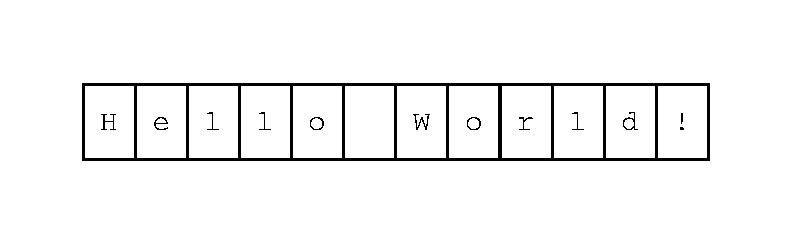
\includegraphics{figures/flat.pdf}
\end{figure}

Indépendamment de l'implémentation, qu'elle soit similaire à C, ou à Pascal, la structure possède
ses avantages et inconvénients.

Avantages:
\begin{enumerate}
	\item accès indexé constant à un codet;
	\item bonne performance en cache.
\end{enumerate}

Inconvénient:
\begin{enumerate}
	\item besoin d'espace contigu.
\end{enumerate}

Du fait de cet inconvénient, cette représentation des chaînes de caractères peut
dégénérer assez rapidement en terme d'espace et de coût.
En effet, lorsqu'une chaîne de caractères mutable est pleine, il faut réallouer
un espace plus grand et copier les anciennes données vers le nouvel espace.
Cette opération est peu coûteuse sur les chaînes de caractères de petite taille, les
coûts d'allocation et de copie étant négligeables dans ce cas.
En revanche cela peut dégénérer sur de grandes chaînes de caractères.

Ce problème des chaînes plates est encore aggravé avec l'immutabilité,
dans la mesure où la moindre opération de mutation entraîne une
réallocation complète de la chaîne.
L'impact de cette ré-allocation est généralement réduit dans les implémentations
de \texttt{buffer} par le biais de sur-allocations.
L'approche ici est de pré-allouer une quantité de mémoire supérieure à ce qui est
demandé pour amortir les coûts de l'allocation et de la copie sur un nombre suffisant de
concaténations.
La performance exposée ici est dans le cas général, suffisante pour les opérations
de concaténation multiples, les cas dégénératifs (insertion non-terminale d'une
chaîne) exposés par cette solutions étant rares, il est par conséquent peu fréquent
que les bibliothèques proposent une solution efficace et standard à ces problèmes.

\subsection{Liste chaînée}

Dans le monde fonctionnel, la représentation en tableau est bien souvent éclipsée
par la liste chaînée, représentée dans la figure~\ref{llistexample}.
Les langages hérités de Lisp utilisent cette structure.
C'est également le cas d'Haskell.

\begin{figure}
	\caption{Exemple de liste chaînée}
	\label{llistexample}
	\centering
	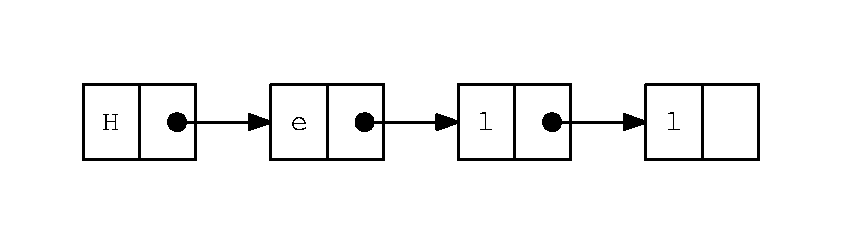
\includegraphics{figures/linked_list.pdf}
\end{figure}

Elle possède certains avantages par rapport à un tableau, notamment la capacité d'extension
en temps constant\footnote{Lorsque la mutabilité des structures est supportée, sinon l'opération
effectuée en temps linéaire.}.
Notons que si l'opération d'insertion s'effectue en temps constant, l'opération de
recherche du point d'accès se fait néanmoins en temps linéaire, à l'exception éventuellement
des extrêmités.
Il est également possible d'amortir l'opération en temps constant par le
biais d'un système de cache.

La représentation est néanmoins peu populaire dans les langages procéduraux et à objets, le
désavantage majeur de la solution est sa faible performance dans le cas de sous-chaînage,
ce dernier nécessitant la réallocation de chaque caractère afin de produire une nouvelle
chaîne.
L'itération, bien que théoriquement aussi performante qu'une approche par tableau, est mise à
mal par les caractéristiques des processeurs modernes de par son impossibilité à être
mise en cache efficacement.
La problématique de l'utilisation mémoire est aussi à prendre en compte.
En effet, chaque caractère est stocké dans un maillon; sa taille est donc la somme de
la taille du caractère et d'un un pointeur, au minimum.

\subsection{Corde}

Une autre alternative existe: la \texttt{corde} \cite{Boehm95}, illustrée dans la figure~\ref{ropeexample}.

\begin{figure}
	\caption{Exemple de corde}
	\label{ropeexample}
	\centering
	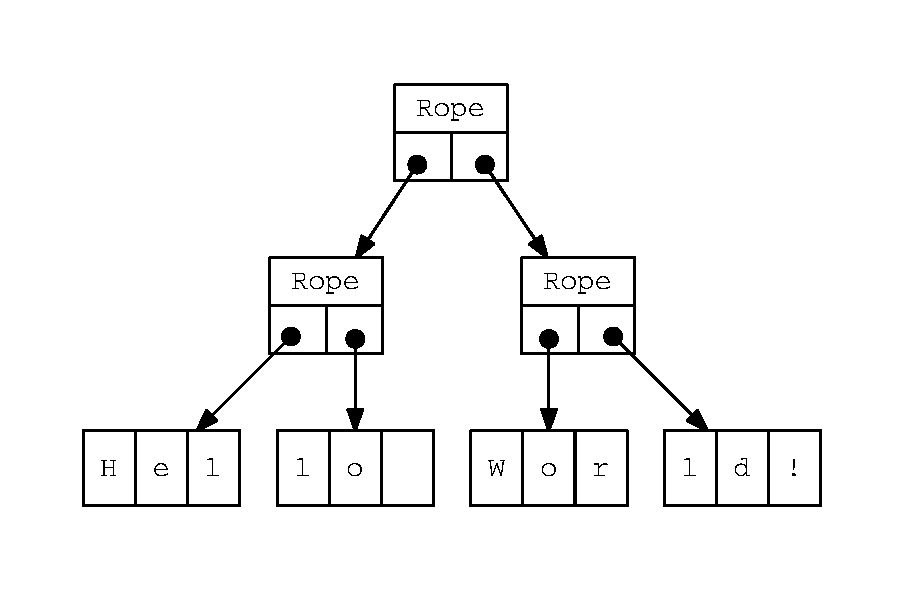
\includegraphics{figures/rope.pdf}
\end{figure}

Une corde est un arbre binaire accessible par index.
Chaque noeud de l'arbre est un noeud représentant une concaténation.
Les \texttt{feuilles} quant à elles sont des chaînes de caractères plates.

La structure propose de réduire la complexité d'opérations comme la concaténation à un
temps constant en remplacant l'allocation et la copie du contenu des chaînes par
la création d'un noeud de concaténation.
Cet avantage est néanmoins à nuancer du fait de la nécessité de ré-équilibrer la corde
périodiquement pour assurer les bonnes performances de la structure.
Elle permet également de réduire la complexité temporelle des opérations comme
l'insertion dans une chaîne à O(log(n)).
Cette opération s'effectue en trois étapes:

\begin{enumerate}
	\item le parcours jusqu'a la feuille à séparer (O(log(n)) si la corde est équilibrée);
	\item la séparation en deux parties à l'index d'insertion (complexité équivalente à deux substring + deux allocations de noeud de concaténation);
	\item la ré-écriture du parcours jusqu'a la racine (O(log(n))).
\end{enumerate}

Avantages:
\begin{enumerate}
	\item concaténation efficace en temps et en espace;
	\item potentiel de partage des feuilles (moins d'allocations).
\end{enumerate}

Inconvénients:
\begin{enumerate}
	\item accès en O(log(n)) aux feuilles de la chaîne;
	\item besoin de garder la structure équilibrée pour maintenir la complexité en O(log(n)).
\end{enumerate}

Malgré son introduction il y'a près de 20 ans, cette structure n'est
jamais devenue populaire, et a fini par tomber dans les limbes.
Cependant, il y'a eu des cas de re-découverte dans lesquels les cordes
étaient plus pertinentes à utiliser que des chaînes plates comme les éditeurs de
texte \cite{inria_rope}.

\subsection{Conclusion}

Parmi les langages modernes, peu proposent une alternative à la chaîne plate comme structure de
données pour les chaînes de caractères.
En dehors des langages à objets ou procéduraux, la liste chaînée est privilégiée dans les
langages fonctionnels, qui eux aussi évitent la corde.
Nit est donc un des rares langages à intégrer les cordes dans leur bibliothèque standard.
Julia~\cite{bezanson2012julia} propose également les cordes, cependant elle est dépréciée\footnote{
\url{https://github.com/JuliaLang/julia/blob/86cd5ea3c61426ebddd1d3809ffa869d6726fb30/base/deprecated.jl}}
pour des raisons de peformance, ceux-ci ne proposant pas de système de conversion, elle doit être
explicitement instanciée par les utilisateurs.
Ces derniers en abusant, les performances diminuaient, ce qui a mené à sa dépréciation.

\section{Codage}

Les chaînes de caractères en tant que telles sont des séquences de caractères.
Selon le codage utilisé, la définition de caractère peut varier.

À l'origine, il n'existait pas de standard pour la représentation des caractères.
Chaque système possédait sa variation d'une correspondance entre données binaires
et caractères.
À l'apparition des cartes perforées, les codages des caractères étaient propriétaires.
Chaque producteur de cartes possédait son propre codage, ce qui empêchait
l'interopérabilité entre différents fabricants.

Simultanément, en 1963, deux codages sont apparus et seront la base des deux grandes
familles de codages ayant façonné l'histoire de l'informatique: \textit{American Standard
Code for Information Interchange} (ASCII) \cite{ASA63} et \textit{Extended Binary Coded Decimal
Interchange Code} (EBCDIC) \cite{amdahl1964architecture}.
Le premier étant un effort de l'\textit{American Standards Association} (ASA), ancêtre de 
l'\textit{American National Standards Institute} (ANSI) et devenant un standard de facto au
départ, avant sa normalisation par ISO/IEC via l'ISO/IEC-646 \cite{ISO72}.
L'autre étant une extension du codage propriétaire d'IBM, \textit{Binary Coded Decimal},
déjà utilisé sur les cartes perforées du fabricant.

ISO/IEC-646 marque le début de la standardisation des codages de caractères en informatique.
Il définit une multitude de codages sur 7 bits pour les caractères de l'alphabet latin.
Il est suivi, dans les années 1980 des variantes de l'ISO/IEC-8859 ou ECMA-94 \cite{ECMA94} du côté européen.

Les limites de l'ASCII ou de l'ISO-8859 se sont vite fait ressentir dans les pays étrangers, si bien
qu'une multitude de codages ont commencé à appraître dans le monde entier; JIS X 208 \cite{JISX208}
pour le Japon, GOST 10859 \cite{GOST64} pour l'URSS, remplacé plus tard par KOI-8 \cite{KOI8} et ses
dérivées, GB2312 \cite{GB2312} pour la Chine, les variantes de Big5 \cite{big5cite} pour Taiwan,
Hong-Kong et Macau, etc.

La multitude de codages rendait l'échange d'information entre les pays difficile, voire dans certains cas
à l'intérieur d'un même pays, ce qui motiva la création d'Unicode \cite{Unicode91}.
En conjonction avec l'ISO/IEC, le consortium Unicode et IEEE partici-pèrent à l'élaboration
d'\textit{Universal Character Set} (UCS) \cite{UCS1993}.

\subsection{UCS-2}

Quand les travaux sur Unicode ont commencé, en 1988, le standard à venir ne concernait
qu'un codage et une table de caractères; les deux étaient confondus \cite{Unicode88}.
L'espace prévu par Unicode pour décrire les caractères supportés était de 16 bits (65536 valeurs).
Chaque valeur définie dans le standard est appelée selon Unicode un \texttt{point de code}.
Pour coder cette information, UCS-2 (alors appelé Unicode) est décrit dans la première version du
standard \cite{Unicode91}.

Il s'agit d'un codage à longueur fixe, à l'instar de ISO-646 ou ISO-8859, chaque valeur possède
un caractère associé.
Du fait de ses codets de 16 bits, UCS-2 est vulnérable aux problèmes de boutisme, contrairement
aux codages utilisant l'octet comme codet.
Pour palier ce problème dans les fichiers, Unicode préconise l'utilisation d'un
BOM\footnote{Byte Order Mark, point de code 0xFEFF déterminant le boutisme d'un bloc de texte Unicode.}
dans les fichiers Unicode.
Si le fichier est codé en UTF-16, les deux premiers octets seront soit \texttt{0xFFFE} dans le cas de
petit-boutisme ou \texttt{0xFEFF} dans le cas de gros-boutisme.
À la publication d'ISO-10646 dans sa première version \cite{UCS1993}, il est l'un des deux codages couverts
par la norme, l'autre étant UCS-4.

\subsection{UCS-4}

UCS-4 est similaire à UCS-2 dans le sens où il propose un codage de longueur fixe.
La différence est que UCS-4 propose des codets de 32 bits au lieu de 16 bits.
La raison à cela est un conflit d'opinion entre le consortium Unicode et
le sous-groupe d'ISO/IEC responsable de la normalisation d'UCS.
Le Consortium Unicode était convaincu que 16 bits suffiraient pour coder l'intégralité
des caractères du monde entier, là où ISO/IEC proposait de normaliser un espace de
données de 32 bits coupé en plans de 65536 valeurs.
Pour les mêmes raisons qu'UCS-2, cette représentation est vulnérable aux problèmes de
boutisme.

Lors de la fusion des deux normes, les deux codages ont été ajoutés aux documents.
Unicode ne spécifiait que les 65536 premières valeurs et ISO/IEC supportait l'ajout
ultérieur de nouvelles valeurs dans l'espace disponible.

\subsection{UTF-8}

UTF-8 est un des codages définis par Unicode et ISO/IEC-10646.
La première version a été produite par Rob Pike et Ken Thompson dès
1992 et implémentée dans le système d'exploitation de recherche Plan9 \cite{Plan9}.

UTF-8 a été créé pour deux raisons principales; la première étant la rétro-compatibilité avec
ASCII et les chaînes de caractères C, terminées par un octet nul (0x00).
La deuxième raison est que les concepteurs d'UTF-8, conscients du différend de point
de vue entre Unicode et ISO/IEC, ne voulaient pas se borner aux 16 bits définis par
Unicode et étaient mécontents d'UCS-4 à cause de la perte d'espace occasionnée par les codets de 32 bits.
UTF-8 est donc un codage à longueur variable ayant pour codet l'octet.
Il est capable de coder l'intégralité des points de code supportés par ISO/IEC 10646.

Chaque point de code est codé sur une séquence de 1 à 6 octets.
Le premier octet de la séquence détermine la longueur de la séquence, par la suite,
chaque octet de la séquence doit respecter le motif '10'.
Le tableau~\ref{utf8_sequences} montre l'organisation des séquences UTF-8.

\begin{table}
	\caption{\label{utf8_sequences}Organisation des séquences UTF-8}
	\centering
	\begin{tabular}{llllll}
		\hline
		Point de code & Glyphe & Octet 1 & Octet 2 & Octet 3 & Octet 4\\
		\hline
		0x41 & A & 0x41 & & & \\
		0xC9 & É & 0xC3 & 0x89 & & \\
		0x3042 & {\fontspec{WenQuanYi Micro Hei}あ} & 0xE3 & 0x81 & 0x82 & \\
		0x1F60A & {\fontspec{DejaVu Sans}😊} & 0xF0 & 0x9F & 0x98 & 0x8A \\
		\hline
	\end{tabular}
\end{table}

\subsection{UTF-16}

À la version 2.0 d'Unicode, le nombre total de caractères définis a dépassé les 65536 prévus
à la base par Unicode.
Pour palier ce problème, le consortium Unicode a fait évoluer UCS-2 en UTF-16.

Le codage fonctionne par un systèmes de paires complémentaires et est capable de coder un total
de 1 114 111 caractères.
À la date de rédaction de ce mémoire, 120 737 points de code sont assignés \cite{Unicode8}.
De ce fait, le standard est limité depuis à ce nombre de points de code.
UTF-8 n'ayant plus besoin de supporter 2 milliards de points de code, sa spécification est simplifiée
et le nombre maximal de codets est limité à 4.
Des points de codes compris entre 0xD800 et 0xDFFF sont réservés pour coder les paires complémentaires
et ne sont valides qu'en UTF-16.

Le tableau~\ref{unicode_sequences} montre les différentes représentations possibles du caractère {\fontspec{DejaVu Sans}😊} 
en fonction des différents codages Unicode.

\begin{table}
	\caption{\label{unicode_sequences}Représentation du caractère {\fontspec{DejaVu Sans}😊} dans les codages Unicode}
	\centering
	\begin{tabular}{lllll}
		\hline
		Codage & Octet 1 & Octet 2 & Octet 3 & Octet 4\\
		\hline
		UTF-8 & 0xF0 & 0x9F & 0x98 & 0x8A \\
		UTF-16 BE & 0xD8 & 0x3D & 0xDE & 0x0A \\
		UTF-16 LE & 0x3D & 0xDE & 0x0A & 0xDE \\
		UTF-32 BE & 0x00 & 0x01 & 0xF6 & 0x0A \\
		UTF-32 LE & 0x0A & 0xF6 & 0x01 & 0x00 \\
		\hline
	\end{tabular}
\end{table}

\subsection{Support d'Unicode dans les langages de programmation}

Parmi les langages modernes, presque tous possédant des sémantiques liées à Unicode dans leur
gestion des chaînes de caractères.

Le niveau de support d'Unicode varie selon les langages, certains supportent les
opéra-tions de base de façon correcte vis-à-vis du standard.
D'autres supportent les extensions liées aux locales (ce qui est nécessaire pour
le tri par exemple).

Au niveau des codages par exemple, Java et C\# utilisent UTF-16 en interne,
les opérations de modification sont fonctionnelles avec des sémantiques
d'Unicode et offrent également des extensions de locales.

Python, avant sa version 3, offrait deux types de chaînes de caractères.
\texttt{str}, qui est composé de octets arbitraires, et \texttt{unicode}, composé
de codets UTF-16 \cite{PEP100}, ou de codets UTF-32 si l'interpréteur est compilé
pour les utiliser en interne.
Plus tard, une extension des caractères pousse le codage
des chaînes de caractères en UTF-32, si le programmeur le demande
explicitement.
En Python 3, le PEP 393 \cite{PEP393} change l'implémentation interne en codets ISO8859-1,
UTF-16 ou UTF-32 dépendamment du plus grand point de code de la chaîne.

Ruby ne définit pas de codage par défaut pour ses chaînes de caractères,
chacune d'elles possède son propre codage et les opérations qui les
manipulent sont différentes en fonction du codage de la chaîne.
Les deux raisons principales de cette approche sont:
\begin{enumerate}
	\item la réduction du nombre d'opérations de codage/décodage à la lecture ou l'écriture vers un média;
	\item une protection contre les problèmes à long-terme du choix d'un codage unique (dépréciation, évolution
de la norme, etc.).
\end{enumerate}

\subsection{Évolution des opérations avec Unicode}\label{unicode_troubles}

Avant l'arrivée d'Unicode, les opérations sur des chaînes de caractères étaient efficaces du fait
de la simplicité des normes et du codage sous-jacent.
Les comparaisons se basaient sur la valeur du codet, les manipulations pour changer la casse
des caractères se résumaient à des opérations arithmétiques ou des accès à une table.
Unicode vient bouleverser cette sémantique et complexifier l'ensemble des manipulations.

Prenons l'exemple de l'équivalence de chaînes de caractères; l'apparition de caractères combinants
vient complexifier l'opération dans la mesure où les combinaisons de points de code doivent
être résolues avant d'effectuer une comparaison entre deux chaînes (voir tableau~\ref{combining_example}).
Il existe également le problème de caractères isomorphes; des
glyphes\footnote{Représentation graphique d'un signe typographique.} représentant des caractères différents
sont équivalents ou tout du moins très similaires (exemple: le signe d'Angström Å et le A-Ring utilisé
dans les alphabets nordiques Å).
L'ensemble de ces cas doivent être pris en compte pour assurer une comparaison respectant le standard
Unicode.

\begin{table}
	\caption{\label{combining_example}Exemple de caractères combinants à glyphe équivalent}
	\centering
	\begin{tabular}{lll}
		\hline
		Glyphe & Point de code & Code Combinant \\
		\hline
		Å & U+00C5 &   \\
		Å & U+0041 & U+030A \\
		Å & U+212B &  \\
		\hline
	\end{tabular}
\end{table}

Il existe également une deuxième façon spécifiée de comparer deux chaînes: la compa-tibilité.
Il s'agit de permettre la prise en compte de versions sémantiquement égales mais graphi-quement différentes
d'un même caractère.
Sous cette forme de comparaison, les chaînes \og H2O \fg{} et \og H$_{2}$O \fg{} doivent être considérées
comme égales.

Si l'égalité canonique est prévisible et fiable, l'ordonnancement de caractères est autre-ment plus complexe
car dépendant de la locale, les lettres doivent être ordonnées différemment dans certains contextes.
Par exemple: \og ll \fg{} va être considéré comme deux lettres dans les pays d'europe, sauf en espagne où
\og ll \fg{} est
une ligature\footnote{Fusion de deux graphèmes d’une écriture pour n’en former qu’un seul nouveau.} considérée
comme une lettre indépendante, qui possède sa rubrique dans un dictionnaire ou un bottin téléphonique,
située entre le \og l \fg{} et \og m \fg{}.
Il existe également des cultures où il n'existe pas d'ordre officiel de comparaision (ex: Japon) et d'autres
où plusieurs ordres sont disponibles (ex: Allemagne).

Ces problèmes de sémantique amènent des problèmes de recherche de motifs: veut-on se baser sur
l'équivalence canonique ou sur de la compatibilité lors de la recherche? À quel point veut-on sacrifier de
la performance pour de la simplicité d'utilisation?

Des modifications comme \texttt{trim}\footnote{Suppression des caractères d'espacement au début et à la fin d'une chaine de caractères.}
deviennent également complexes dans la mesure où les espaces ne sont
plus confinés à un espace restreint comme ASCII ou ISO-8859 l'avaient défini, mais à toute la table
Unicode.
De plus, certains caractères sont reconnus comme des caractères d'espacement, mais n'en ont pas
nécéssairement l'air: U+1680 par exemple, est un caractère d'espacement en alphabet Ogham, un alphabet runique
irlandais, dont le glyphe ressemble à un \texttt{-}.

Les opérations de modifications de caractères sont elles-aussi dépendantes de la locale.
Par exemple le caractère \og i \fg{} va se transformer en \og I \fg{} pour la majorité des utilisateurs,
sauf en locale Turque, ou il sera représenté par le caractère \og İ \fg{}.
Par ailleurs, les opérations de modification de casse sont non symétriques.
En allemand, le caractère \og ß \fg{} se transforme en \og SS \fg{} une fois en majuscule, qui eux, se transforment
en \og ss \fg{} une fois en minuscule.
Cette sémantique pose également un problème pour les API retournant un caractère lors de
l'opération dans la mesure ou un caractère unique peut se transformer en une chaîne de
caractères.

\subsection{Définition: caractère}

Dans la mesure où une chaîne de caractères est une suite de caractères,
un point sur lequel tous les langages pourraient à priori sembler
d'accord est la notion même de caractère.

En réalité, il n'existe pas de consensus concernant le caractère.
Il peut être une entité complètement différente d'un langage
à l'autre.
Parfois pour des raisons historiques (Java et ses codets UTF-16), parfois
de vision (Go avec UTF-8 ou Swift avec ses Extended Grapheme Clusters), voire dans
certains cas la notion est inexistante (Ruby, Python, etc.).

C et C++ considèrent des chaînes de caractères comme des
tableaux d'octets terminés par un octet 0x00.
Avec l'arrivée d'Unicode, un type \texttt{wchar\char`_t} a été ajouté au standard
pour supporter les codages comme UTF-16 ou UTF-32.
Cet ajout n'est cependant pas exempt de défaut et certains projets comme
GNU libunistring\footnote{The \texttt{wchar\char`_t} mess - \url{https://www.gnu.org/software/libunistring/manual/html_node/The-wchar_005ft-mess.html}.}
critiquent avec véhémence le type de données du fait de son manque de standardisation,
de sa faible utilité dans les implémentations limitant sa taille à 16 bits, ainsi que
de la fragilité des API associées.

Des langages plus haut-niveau comme Java \cite{java_spec} définissent leurs caractères comme
des codets UTF-16.
Ils ont une taille fixe de 16 bits et la gestion des paires d'extension est laissée
au programmeur.
C\# \cite{csharp_spec} et Javascript \cite{ecmascript_spec} le définissent de façon similaire.

Go \cite{goref} définit un concept analogue à un point de code nommé
Rune, à l'instar des Runes défninies par Plan9 \cite{Plan9}.
Leurs chaînes de caractères sont en fait des tableaux d'octets et ils
possèdent des opérations pour les traiter comme de l'UTF-8, 16 ou 32, le codage des chaînes
étant UTF-8 par défaut.

Swift \cite{swiftref} est un des rares langages statiquement typés et compilés à définir un
caractère comme une structure non primitive.
En Swift, un caractère est défini comme un ensemble étendu de graphèmes \cite{Unicode8}.
Il s'agit d'une séquence d'un ou plusieurs points de code, qui
combinés, produisent un caractère lisible par un être humain.

D'autres langages comme Ruby ou Python sont complètement dépourvus de la notion de
caractère, et un accès à une chaîne de caractères renvoie systématiquement
une sous-chaîne.
Perl, dans sa version 6, définit plusieurs niveaux d'accès aux éléments d'une chaîne:
octets, points de code, graphèmes.

\subsection{Conclusion}

La notion de codage est variable selon les langages (voir tableau~\ref{coding_recap}).
Certains définissent un codage par défaut, d'autres en supportent explicitement
plusieurs, voire certains ne font pas de distinction entre objet binaire et chaîne
de caractères.
De cette notion découle directement la notion de caractère, elle aussi ambigüe.

\begin{table}
	\caption{\label{coding_recap}Codage, selon les langages}
	\centering
	\begin{tabular}{llllll}
		\hline
		& Aucun & Variable & UTF-8 & UTF-16 & UTF-32 \\
		\hline
		Java & Non & Non & Non & Oui & Non \\
		C\# & Non & Non & Non & Oui & Non \\
		C & Oui & Non & Non & Non & Non \\
		Ruby & Non & Oui & Oui (défaut) & Oui & Oui \\
		Python & Non & Oui & Non & Oui (UCS-2) & Oui \\
		Perl & Non & Oui & Oui (défaut) & Oui & Oui \\
		Nit & Non & Non & Oui & Non & Non \\
		Swift & Non & Non & Non & Oui & Non \\
		Go & Non & Oui & Oui (défaut) & Oui & Oui \\
		\hline
	\end{tabular}
\end{table}

\section{Opérations primitives}

Nous identifions trois opérations primitives des chaînes de caractères dans cette étude.
Ces trois opérations serviront à implémenter l'ensemble des opérations sur des chaînes
de caractères et détermineront la complexité globale sur ces dernières.

\subsection{Concaténation}

Le processus de concaténation est la création d'une nouvelle chaîne de caractères à partir
de deux morceaux, eux-mêmes des chaînes de caractères indépendantes.
L'opération est effectuée de plusieurs façons dans les langages actuels.

Java et C\# par exemple travaillent avec des chaînes de caractères plates, l'utilisation de
l'opérateur de concaténation provoque l'allocation d'un nouvel espace pour le
contenu des deux chaînes et la copie avant de stocker cet espace dans un nouvel objet.
Il est à noter que dans ces deux langages, le cas où plusieurs concaténations sont syntaxiquement effectuées
à la suite est optimisé et les concaténations individuelles sont remplacées par un \texttt{buffer}
et des ajouts mutables.

Ruby possède plusieurs façons de concaténer des chaînes, l'opérateur + ou l'opérateur \textless\textless.
La différence entre les deux est que \textless\textless est mutatif (et donc non-sûr
dans la mesure où un objet peut être \texttt{frozen}\footnote{Rendu immutable par la fonction freeze du langage.})
là où + crée une copie.
De par son caractère mutatif en revanche, \textless\textless  est plus efficace.

Des langages comme Python, ne possèdant pas de chaînes mutables,
conseillent de passer par des tableaux de chaînes dans le
cas de concaténations multiples, puis de joindre l'ensemble.
Il existe également un opérateur + pour la concaténation simple.

\subsection{Accès indexé}

Une autre opération fréquente sur des chaînes de caractères est l'accès à un caractère
de la chaîne.
Dépendamment de la définition de caractère, l'opération change de sens.

La définition de Java selon laquelle un caractère est un codet UTF-16 lui permet d'offrir
au programmeur une complexité temporelle en O(1) pour l'accès à un caractère, peu importe
sa position dans la chaîne.
Le problème de cette approche est que selon Unicode, un point de code est potentiellement
codé sur 32 bits, laissant au programmeur le soin de gérer les paires complémentaires.
Il s'agit d'un problème récurrent dans les implémentations des chaînes utilisant UTF-16
(C\# et Python 2.x souffrent du problème par exemple),
qui peut sembler fonctionnel tant que le texte contient uniquement des caractères du 
BMP\footnote{Basic Multilingual Plane, les 65535 premiers caractères de la norme Unicode,
représentant les langues vivantes actuelles.}; le cas le plus fréquent.
Cependant, lorsque le texte contient des caractères en dehors de ce plan, un accès indexé
ne renverra qu'une partie de ce caractère, provoquant des comportements bogués.

Des langages comme Go fournissent une interface de récupération de Runes respectant
le standard établi par Unicode.
En UTF-8 ou UTF-16, les codages étant de longueur variable, l'accès à un caractère
est donc en complexité O(n).
UTF-32 étant également supporté par le langage et de par son statut de codage à
longueur fixe, il offre un accès en temps constant.

Des langages comme Swift, traitant les caractères comme des graphèmes, sont
obligés de gérer les possibilités de points de code combinants\footnote{Façon de gérer les caractères avec diacritiques par un système de combinaison.}
suivant un point de code quelconque.
Une première opération de récupération d'un caractère est effectuée en un premier temps, de complexité
temporelle linéaire.
S'en suit une phase de lookahead pour déterminer la présence de caractères combinants.
Cette opération est potentiellement dégénérative, Unicode ne limitant pas le nombre de
caractères combinants après un caractère de base.

\subsection{Sous-chaînage}

La dernière opération fondamentale des chaînes de caractères est la production de
sous-chaînes.
Lorsque l'on travaille avec des chaînes de caractères, il est souvent nécessaire
de travailler sur des sous-parties d'une plus grande chaîne.
La façon simple de procéder est d'en extraire une sous-chaîne indépendante sur
laquelle effectuer un traitement ultérieur.

Il existe deux façons principales de produire des sous-chaînes: par copie ou par référence.
La copie est utilisée en C\# par exemple; à chaque appel à \texttt{substring}
un nouvel espace est alloué et le contenu de la chaîne est copié, occasionnant une
complexité temporelle et spatiale de O(n).
L'avantage de la manoeuvre est que la chaîne de base n'est plus référencée et peut être
désallouée de façon sûre.
Le principal désavantage vient des manoeuvres de réallocation et copie qui dégénèrent
sur de grandes chaînes.

Java est également de ces langages à allouer de nouvelles chaînes à chaque appel à
\texttt{substring}.
Cependant, ce n'est le comportement par défaut que depuis la version 7 update 6.
Avant cela, les données de la chaîne étaient partagées entre plusieurs instances,
le début de la chaîne était stocké dans la structure elle-même sous la forme d'un
décalage et d'une longueur pré-définie.
La raison de ce changement est au niveau de l'utilisation de la mémoire, les sous-chaînes
empêchant le ramassage de la chaîne parente, si cette dernière est large, elle peut
occasionner des problèmes de capacité mémoire.
Un autre point invoqué est la non-applicabilité de la complexité O(1) sur une chaîne
de petite taille; essentiellement, une allocation et une copie pour un petit espace
de données est négligeable par rapport au
maintien des indices et aux coûts additionnels des opérations
dans le cas d'une chaîne partagée.

\section{Conclusion}

Ce chapitre présente les différents points de variabilité des chaînes de caractères dans les
langages de programmation.
Qu'il s'agisse de différences structurelles, de codage ou de mutabilité; chaque langage possède
une idée qui lui est propre de la chaîne de caractères.
Ces choix possèdent tous des avantages et des inconvénients, et il n'existe pas, ni n'existera
un jour, de chaîne de caractères parfaite, dépourvue d'inconvénients.
En revanche, il est possible de limiter les inconvénients de chaque approche, tout en
gardant les avantages de chaque représentation.
Le prochain chapitre présente la solution que nous avons implémentée en Nit, et qui représente
selon nous un bon compromis entre tous les points soulevés ici.

\chapter{Proposition de modèle de représentation des chaînes de caractères et contributions}\label{solution_chap}

Les chaînes de caractères sont des structures de données primordiales pour un langage de programmation.
Tous les langages proposent un modèle, chacun avec ses avantages et ses inconvénients.
Certains privilégient la facilité d'utilisation et la parallélisation via des chaînes immutables,
d'autres privilégient la rapidité via des chaînes mutables.
Au niveau de la structure de données, le tableau de caractères est la structure la plus fréquente
dans les langages impératifs et à objets.
Cependant, les problèmes de la structure, détaillés en section~\ref{state_flatstr_prez}, en
ce qui concerne le passage à l'échelle nous font demander s'il n'est
pas possible de l'améliorer, tout en gardant l'utilisation aussi simple que possible du point
de vue des utilisateurs du langage.

Ce chapitre présente le modèle des chaînes de caractères en Nit, 
les modifications que nous avons apporté à la bibliothèque standard, pourquoi nous avons pris
ces décisions et quels sont les travaux restants.

\section{Ancien modèle}

\subsection{Les chaînes sous forme de tableau}

Au début de ce travail, les chaînes de Nit étaient uniquement des tableaux de caractères.
La définition de caractère selon le langage était calquée sur celle de C: un caractère Nit
était un \texttt{char} C, c'est à dire un octet.
Les manipulations étaient orientées octet et le contenu d'une chaîne n'était pas partagé,
la production d'une sous-chaîne de caractères entraînait l'allocation et la copie partielle du
contenu de la chaîne d'origine.
Les chaînes de caractères étaient des enveloppes autour d'un \texttt{char*} natif: \texttt{NativeString}
(voir figure~\ref{oldmodel}).

Il existait deux alternatives dans la construction des chaînes de caractères:

\begin{enumerate}
	\item\texttt{String}: chaîne de caractères immutable.
	\item\texttt{Buffer}: chaîne de caractères mutable, notamment utilisée pour la concaténation et les modifications efficaces.
\end{enumerate}

\begin{figure}
	\caption{Ancien mod\`{e}le des chaînes de Nit}
	\label{oldmodel}
	\centering
	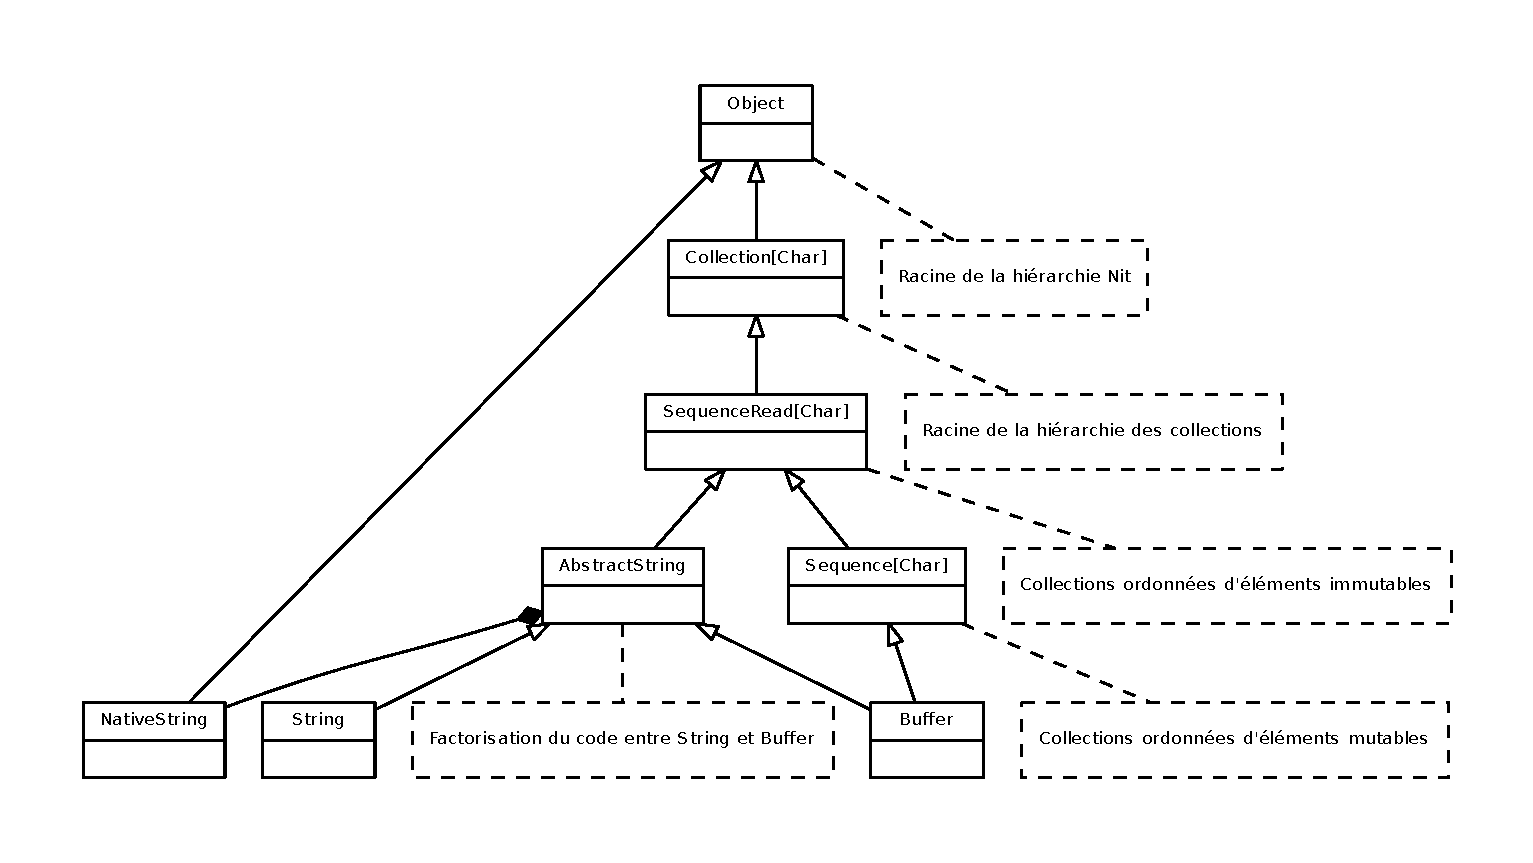
\includegraphics[angle=90, scale=0.75]{figures/old_model.pdf}
\end{figure}

Malgré le non-support d'un codage multilingue, l'ancien modèle possédait des avantages certains:

\begin{enumerate}
	\item Les accès à un caractère étaient effectués en temps constant.
	\item La structure en \texttt{char*} permettaient un passage facile et peu coûteux vers les morceaux de code C.
	\item Le modèle était simple à comprendre.
\end{enumerate}

Cependant, malgré ces avantages, il possèdait toutes les limitations dûes aux chaînes plates,
qui malheureusement ne peuvent être résolues simplement en optimisant les opérations effectuées sur ces
dernières.

\begin{enumerate}
	\item Pas de résistance face aux traitements sur de longues chaînes.
	\item Cas dégénératifs lors de concaténations de grandes chaînes.
\end{enumerate}

\subsection{Codage}\label{codage_ancien}

Les chaînes de caractères en Nit étaient anciennement de simples séquences d'octets, aucune
information de codage n'était disponible.
L'ensemble des opérations disponibles se basaient sur les sémantiques de l'ASCII, et tous les caractères
en dehors de cette zone étaient ignorés, menant parfois à des résultats erronés du point de vue de
l'utilisateur.

En effet, un simple programme comme celui-ci:

\begin{verbatim}
var s = "être"
for c in s.chars do printn "{c}-"
\end{verbatim}

Produisait le résultat erroné: \texttt{{\fontspec{DejaVu Sans}�}-{\fontspec{DejaVu Sans}�}-t-r-e-}

Dans la mesure où ASCII n'est pas le seul codage capable de représenter des chaînes de caractères en
utilisant l'octet comme codet, aucune manipulation n'était véritablement sûre et du texte codé dans un
codage possédant une représentation similaire (KOI-8, GOST-10859, etc.) risquait d'être corrompu.

\section{Nouveau modèle}

\subsection{Codage}

Du fait des limitations présentées en~\ref{codage_ancien}, nous avons changé les chaînes Nit
en séquences de points de code, codées en UTF-8.
Il est désormais possible d'accéder indépendamment aux octets ou aux points de code.

Le support de ces opérations nous permet, sur le morceau de code développé en~\ref{codage_ancien},
de produire le résultat attendu communément: \texttt{ê-t-r-e-}

Les chaînes sont également nettoyées lors du passage d'un objet binaire à une chaîne de caractères de façon
à ce qu'elle ne contienne que des séquences UTF-8 valides.
Par \og nettoyées \fg{}, nous entendons que les séquences UTF-8 invalides sont remplacées par le
caractère de remplacement Unicode {\fontspec{DejaVu Sans}�} (U+FFFD).
Une séquence UTF-8 invalide peut avoir plusieurs formes, il peut s'agir de séquences incomplètes,
d'octets invalides dans un point de code, ou de séquences trop longues.
Par exemple, une séquence \texttt{0xC0 0xAF} est considérée comme trop longue pour représenter
le caractère \texttt{/}, et sa véritable valeur devrait être \texttt{0x2F}.

Cette opération est obligatoire selon le standard Unicode pour assurer une bonne compatiblité
avec les séquences de texte en UTF-8.
Les bibliothèques n'effectuant pas ce type de manipulations s'exposent potentiellement à des soucis de sécurité.
Une vulnérabilité de ce style était présente en PHP par exemple via la fonction \texttt{$mysql\_real\_escape\_string$}.
En injectant une séquence trop longue, la fonction de validation ne nettoie pas le \texttt{'}, et
le caractère qui aurait du être rejeté est accepté.
Cette faille permettait à un tiers malveillant d'injecter du code SQL arbitraire dans une requête.

\subsection{Cordes}

En Nit, nous utilisons les cordes en conjonction des chaînes plates pour plusieurs
raisons.

Le fait qu'aussi bien en UTF-8 qu'en UTF-16, l'accès aux caractères s'effectue de façon linéaire\footnote{Note:
Des langages comme Java et C\# proposent un accès en temps constant en UTF-16, mais l'accès est
non-sûr dès lors qu'un caractère hors-BMP est présent.}
permet aux cordes de mitiger l'utilisation de ces codages dans des chaînes de grande taille en réduisant
l'accès à une complexité temporelle de O(log(n)) pour la sous-chaîne contenant le caractère visé,
puis en O(n) sur une feuille\footnote{Une feuille est une chaîne plate présente à l'extrêmité d'une corde.}.
Cette complexité suppose que la corde sur laquelle l'opération d'accès est effectuée est équilibrée.
En termes d'utilisation mémoire, les cordes sont également avantageuses du fait de la séparation des
chaînes en parties de faible taille.
Le sous-chaînage et des opérations de modification de contenu par exemple permettent de limiter les réallocations
dans les cas où seulement une partie de la chaîne d'origine doit être ré-allouée au lieu de l'ensemble de
la chaîne (i.e. trim, ou seulement la première et la dernière feuille nécéssitent une ré-allocation).

\subsection{L'implémentation en Nit}

Du fait des faiblesses de l'ancien modèle, notamment en termes de passage à l'échelle, nous
proposons un nouveau modèle original pour les utilisateurs du langage, que nous avons
implémenté en Nit.
Il s'articule autour d'une classe abstraite de manipulation du texte: \texttt{Text}.
Un autre changement majeur de ce nouveau modèle en termes d'API vient également de la différenciation
entre les manipulations orientées octet et les manipulations orientées texte.

Deux sous-classes de \texttt{Text} sont exposées: \texttt{String}, pour des chaînes de caractères immutables, et \texttt{Buffer}
pour les chaînes de caractères mutables.
En plus de la différence entre mutable et immutable, deux sous-classes de \texttt{Text} sont
introduites: \texttt{FlatText} et \texttt{Rope}.

\texttt{FlatText} définit la base des chaînes de caractères plates, ce sont des enveloppes autour de tableaux d'octets C.
\texttt{Rope} quant à lui est une structure sous forme de corde, deux implémentations sont disponibles: \texttt{Concat}, une
corde immutable, et \texttt{RopeBuffer}, une version mutable de corde.
Notons que ce dernier est expérimental et était peu performant au moment de rédiger ces lignes.
Une vue d'ensemble de ce modèle est présentée dans la figure~\ref{newmodel}.

Nous proposons de changer de façon transparente au programmeur la représentation interne des
chaînes de caractères pour éviter les cas dégéneratifs exposés par les chaînes plates.
Pour éviter les allocations trop nombreuses et limiter la taille des allocations, qui
deviennent coûteuses passées un certain seuil,
la concaténation de chaînes de caractères est implementée
de façon à produire un noeud de concatenation au lieu de ré-allouer une nouvelle
chaîne plate et d'effectuer une copie de contenu.

\begin{Verbatim}[obeytabs,tabsize=4]
class Text
	fun +(o: Text) do
		var result: String
		if byte_length + o.byte_length > concatenation_seuil then
			result = new Concat(to_s, o.to_s)
		else
			var new_arr = malloc(byte_length + o.byte_length)
			copy_content(new_arr, byte_length, 0)
			o.copy_content(new_arr, o.byte_length, byte_length)
			result = new FlatString(new_arr)
		end
		return result
	end
end
\end{Verbatim}

Cette approche permet également un accès en temps logarithmique au lieu de linéaire
à un caractère abritraire d'une chaîne de caractères.
Si cette faculté est intéressante, elle reste néanmoins anectodique dans la mesure où il s'agit d'un cas de
figure assez rare, les caractères d'une chaîne étant le plus souvent accédés de façon itérative.

Lors de l'introduction d'Unicode dans Nit, il nous est apparu important de faire une distinction claire entre les API
orientées caractères, où un caractère référence le graphème ou le point de code, et les
API orientées sur leur représentation sous-jacente, dans notre cas l'octet.
Il s'agit d'une différence que les implémentations existantes font rarement, et jusqu'à aujourd'hui, parmi les
langages populaires, seuls Perl6, Swift ou Elixir font une réelle distinction entre ces entités.

Pour permettre aux utilisateurs du langage d'accéder au besoin à la représentation sous-jacente,
toutes les représentations de chaînes de caractères disponibles possèdent un systeme de vue sur les différentes
entités du contenu d'une chaîne de caractères: \texttt{Byte} et \texttt{Char}.
Dans le futur, nous souhaitons également proposer une vue orientée \texttt{Graphème} pour accéder au contenu
d'une chaîne de caractères, à l'instar de ce que proposent Perl6 ou Swift.
Présentement, les opérations d'accès par défaut d'une chaîne opèrent au niveau du point de code.
Ce choix est arbitraire, un travail futur permettrait de déterminer si l'accès devrait
se faire au niveau du graphème par défaut, ou non.

\begin{figure}
	\caption{Nouveau mod\`{e}le des chaînes de Nit}
	\label{newmodel}
	\centering
	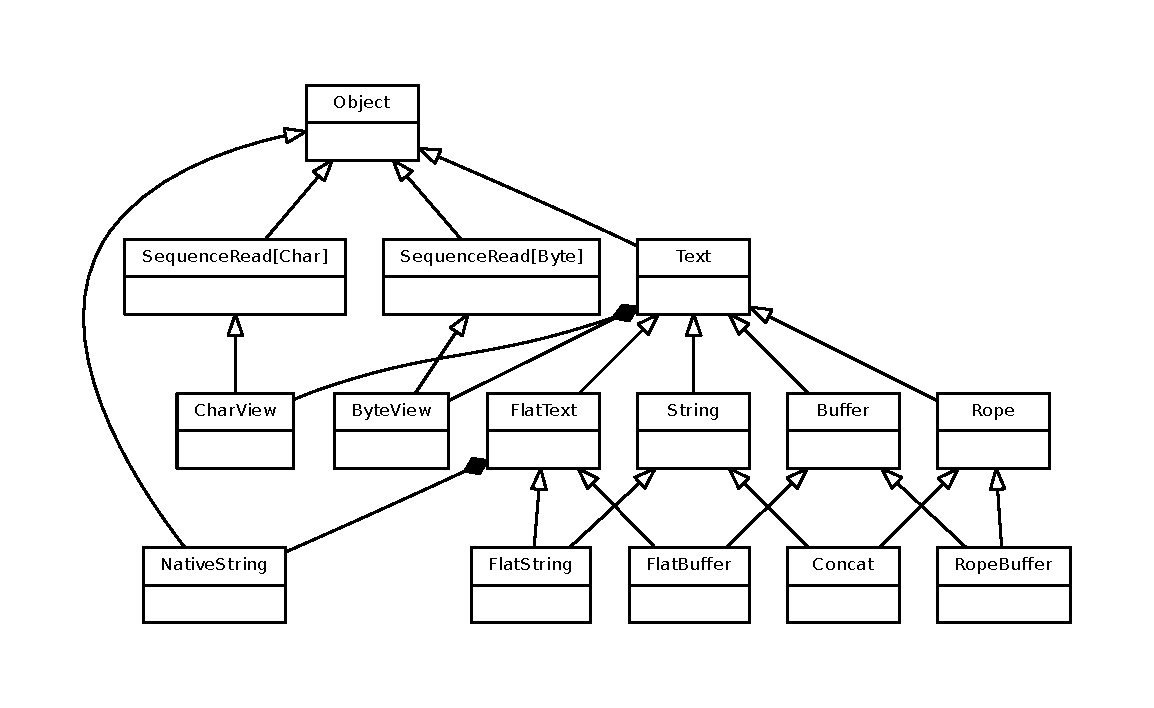
\includegraphics[angle=90]{figures/new_model.pdf}
\end{figure}

La solution que nous présentons expose un modèle complexe à l'implémentation, mais simple à l'utilisation.
Les classes \texttt{FlatString}, \texttt{FlatBuffer}, \texttt{Concat} et \texttt{RopeBuffer} continuent
à être exposées à l'utilisateur pour des raisons de performances dans des cas particuliers.
Cependant, ce dernier continue à interagir avec des chaînes de caractères par le biais des classes abstraites
\texttt{String} et \texttt{Buffer}, ce qui permet de garder une API simple, peu importe la complexité
de la structure sous-jacente.
Notons que l'implémentation de ce modèle a largement été simplifié par le support de l'héritage
multiple en Nit.
S'il est possible d'implémenter un modèle similaire en Java ou dans un autre langage, la réalisation
sera plus complexe et le modèle en découlant comportera plus d'interfaces.

\section{Bibliothèque}

Une première partie du travail en termes d'API consistait à désolidariser les chaînes de caractères
du bloc des collections.
Nous avons pris cette décision du fait de la non-applicabilité de certains services
à des structures comme les chaînes de caractères.

Par exemple, le service \texttt{join} est peu utile dans le cadre d'une chaîne de caractères et avait pour effet
de joindre un motif entre chaque caractère.
D'autres services comme \texttt{sort} par exemple ont peu de sens quand utilisés sur une chaîne,
où le résultat serait d'avoir les caractères triés par ordre lexicographique.

Une partie du travail s'est focalisé sur l'intégration du bloc des cordes.
Nous avons essayé plusieurs alternatives avant de garder l'implémentation actuelle.
Une première était basée sur l'implémentation de SGI Rope, disponible aujourd'hui via les extensions
STL C++ de GNU GCC\footnote{Code disponible à \url{https://gcc.gnu.org/onlinedocs/gcc-4.6.3/libstdc++/api/a01015_source.html}.}.
Cependant, les structures présentées par cette implémentation étaient lourdes de par la création de noeuds
feuille.
Cela nous a contraint à abandonner l'ancien code en faveur de l'actuel, inspiré
de l'implémentation de Boehm, disponible dans le ramasse-miettes du même
nom\footnote{Paquet disponible à \url{https://github.com/ivmai/bdwgc/tree/master/cord}.}.
On notera que les cordes d'SGI comportent deux types de noeud spéciaux en plus de ceux exposés par les notres:

\begin{enumerate}
	\item Noeud fonction: un type de noeud contenant deux références, un vers la corde, et un vers une fonction.
		Ils sont utilisés lors de traitements paresseux sur les cordes. Nit ne permettant pas de représenter et
		d'invoquer une fonction arbitrairement, ils sont laissés de côté dans notre implémentation.
	\item Noeud de sous-chaînage: ces noeuds permettent de créer en temps constant une sous-chaîne en fonctionnant
		d'une façon similaire à la fonction \texttt{substring} de Nit.
		Ils contiennent un pointeur vers une corde, ainsi qu'un index de départ de la sous-chaîne dans cette corde.
		Leur principale raison d'être est leur compatibilité avec les noeuds fonction, afin
		d'effectuer les calculs nécessaires à la production de la sous-chaîne de façon paresseuse.
\end{enumerate}

Une autre partie du travail effectué a été sur l'intégration d'Unicode à la bibliothèque standard.
Il a fallu changer la sémantique et le type associé dans le C généré de \texttt{Char}, dans la mesure
où un caractère a évolué d'octet à point de code.
Ce changement a posé un nombre conséquent de problèmes:

\begin{enumerate}
	\item Clients brisés: certains clients se servaient de chaînes de caractères comme d'un tableau d'octets et se basaient sur l'équivalence entre les chaînes et ces mêmes tableaux; en changeant le type de Char, le code qui dépendait de cette sémantique s'est retrouvé brisé.
	\item Problèmes d'amorçage: Nit possèdant un compilateur autogène, l'ensemble des modifications de la bibliothèque ont des impacts sur la façon dont le compilateur se compile lui-même. En changeant un type primitif, certaines signatures et opérations provoquaient des erreurs dans le C généré par une ancienne version du compilateur, empêchant par ce fait le compilateur de fonctionner.
	\item Problèmes avec les morceaux de code externe: une partie de la bibliothèque de Nit est implémentée directement en C via un mécanisme de FFI\footnote{Foreign Function Interface: Façon d'appeler du code externe depuis du code Nit et vice-versa}~\cite{xymus_memoire}.
		Une partie de ces morceaux de code dépendaient directement de la correspondance entre \texttt{Char} Nit et
		\texttt{char} C.
		En changeant la définition de \texttt{Char} côté Nit, ces utilisations en C doivent changer également et pour
		un certain nombre, le changement ne se limite pas à un simple cast.
\end{enumerate}

Au-delà du changement de sémantique dans les types primitifs,
nous avons changé les opérations de la bibliothèque standard.
Principalement en termes de performance, où des opérations comme
l'accès indexé, qui s'effectuait en temps constant, ont évolué pour s'effectuer en temps linéaire.
Les impacts de ce changement nous ont forcé à inclure un système de cache aux chaînes, de façon à limiter cet impact.
Cependant, il reste des cas où Unicode nous empêche de préserver les mêmes performances.
Un de ces cas est la modification.
En effet, lorsque l'on souhaite remplacer un caractère dans un \texttt{buffer}, il se peut que l'opération doive
s'effectuer en temps linéaire.
Il s'agit là d'un des problèmes majeurs des codages à longueur variable comme UTF-8 ou UTF-16, où le remplacement
d'un caractère peut avoir comme effet de déplacer toutes les données du buffer pour combler ou récupérer
de l'espace.

Par exemple, dans ce morceau de code:

\begin{verbatim}
var b = new Buffer.from("Être")
b[0] = 'E'
\end{verbatim}

Le remplacement de la lettre 'Ê' par 'E' en UTF-8 force le déplacement des caractères suivants de 1 octet vers la
gauche.

Un dernier changement, qui lui aussi a eu des implications sur certains clients, est le nettoyage des objets binaires
lors de leur passage à une chaîne Unicode.
Les bogues liés à ces comportements-là sont bien souvent liés à des programmes similaires à ceux ayant eu des problèmes
lors du changement de sémantique de \texttt{Char}.
En effet, en modifiant le contenu du tableau de caractères sous-jacent à une chaîne, les programmes se servant de
chaînes de caractères comme espace temporaire de stockage des données binaires ont fait face à des corruptions des
données, résultant en des bogues difficiles à tracer pour les personnes non familières avec Unicode.

Ce problème a nécessité l'introduction de nouveaux types dans la bibliothèque standard:

\begin{enumerate}
	\item \texttt{Byte}: Un octet, représenté en Nit. Il s'agit d'un nouveau type primitif, visant
		à remplacer l'ancienne représentation de \texttt{Char}. Les opérations sur les \texttt{NativeString}
		ont toutes évolué pour supporter ce type.
	\item \texttt{Bytes}: Une collection d'octets mutable sous forme plate. Elles peuvent être utilisées
		à la place des anciennes \texttt{String} pour préserver la sémantique orientée octet de ces
		structures dans les cas où le texte n'est pas une priorité. Il est à noter que la conversion
		d'une chaîne de caractères vers un \texttt{Bytes} et vice-versa quand possible, 
		est effectuée via un mécanisme de \textit{copy-on-write}
		de façon à limiter l'impact de la transformation d'une représentation vers l'autre.
\end{enumerate}

En plus des contributions mentionnées plus haut, une preuve de concept d'internationalisation semi-automatique
a été intégrée à la suite d'outils Nit.
Elle a été implémentée sous la forme d'une annotation de module, qui une fois utilisée externalise les chaînes
littérales présentes dans un fichier source dans un fichier \texttt{po}, pour utilisation avec GNU \texttt{gettext}
et remplace leurs utilisations par un appel à \texttt{gettext} pour récupérer la chaîne traduite dans la locale
de l'utilisateur si disponible.
Il s'agit d'une façon standard de faire pour les applications sous Linux.
Il est possible via des modifications mineures de supporter d'autres systèmes d'internationalisation pour d'autres
plateformes, comme le fichier \texttt{R.java}
\footnote{Technique standard en Android pour externaliser des chaînes de caractères littérales à des fins d'internationalisation.}
pour Android par exemple.

\section{Micro-optimisations}

Les changements structurels et de codage nous ont forcé à profiter des attributs physiques de la machine pour
accélérer les opérations fondamentales des chaînes.
Une grande partie de ce travail a été dédié à la micro-optimisation, à l'étude du C et de l'assembleur généré,
ainsi qu'aux caractéristiques physiques des machines sur lesquelles les programmes Nit sont exécutés.
Parmi les optimisations que nous avons implémentées, nous pouvons en citer trois majeures.

\subsection{Accès multiple}

Une façon d'accélérer le parcours des chaînes de caractères est de pré-chercher plusieurs
caractères à la fois et d'effectuer des opérations sur eux. Nous nous servons de cette astuce pour quadrupler la vitesse
de parcours dans des chaînes en ASCII. Il est à noter que cette optimisation peut être améliorée en prenant en compte les
propriétés de différentes architectures. Par exemple, sur un processeur 64-bits, nous pourrions pré-charger 8 caractères
sans surcoût notable par exemple.

\subsection{Caches}

Pour accélérer les opérations courantes sur les chaînes, nous avons mis en place plusieurs systèmes
de cache, aussi bien dans les chaînes plates, que dans les cordes. Dans ces dernières, ils nous permettent de court-circuiter
le parcours de la corde et d'aller chercher directement la feuille sur laquelle effectuer les traitements ultérieurs.
Dans les chaînes plates, ils nous permettent d'effectuer un parcours minimal jusqu'au caractère souhaité.

\subsection{Astuces bas-niveau et langage}

Une façon d'optimiser les opérations effectuées sur des chaînes
a été de réduire le nombre d'appels polymorphes et de court-circuiter au maximum les opérations.
Une autre optimisation, qui induit de la duplication de code, est de micro-optimiser
un maximum de fonctions critiques sur chaque sous-classe de \texttt{Text} pour s'assurer d'avoir
une performance optimale, et ce, peu importe le type de receveur.

Une dernière optimisation que nous avons implémentée, 
qui consiste plus à réorganiser le code, est l'utilisation d'une approche statistique pour
favoriser l'évaluation des options plus fréquentes. Dans chaque méthode critique au niveau de la performance,
nous avons placé les chemins plus fréquents statistiquement pour améliorer les performances au niveau du
matériel, et tirer un maximum de profit de la prédiction de branche et des caches d'instruction.

\section{Conclusion}

Nous proposons dans ce chapitre une solution combinant les cordes et les
chaînes de caractères plates, que nous avons implémentée dans la bibliothèque standard du langage Nit.
Cette solution a pour but d'être efficace dans toutes les situations, y compris dans les cas dégénératifs connus des
chaînes de caractères plates.
Nous souhaitions également qu'elle soit facile à utiliser en transformant de façon transparente les chaînes que
le programmeur crée.
Il s'agit d'une originalité de notre solution, à notre connaissance, aucun langage ne propose un modèle
similaire dans une bibliothèque standard, et toutes les bibliothèques de cordes dans les
langages modernes nécessitent une action spéciale de la part du programmeur pour être utilisées.
Le prochain chapitre de notre étude servira à valider notre solution par le biais de
programmes de mesure de la performance.

\chapter{Variations d'implémentation et mesures de performance}\label{perf_chap}

Les chaînes de caractères étant des structures de données, il existe
plusieurs façons de les implémenter, chacune avec ses avantages
et ses inconvénients.

Au delà même de la structure de base, des variations existent dans
la gestion en interne de ces structures, choix qui auront un impact
sur les opérations primitives de la structure et par extension sur
l'ensemble des services.

Les variations ont ici lieu à plusieurs niveaux:

\begin{enumerate}
	\item Au niveau de la complexité algorithmique
	\item Au niveau de l'affinité des processeurs avec les structures de données
\end{enumerate}

Nous souhaitons mettre l'accent sur la deuxième partie des optimisations,
qui est la plus importante dans notre cas.
En effet, notre solution ayant pour but d'être utilisée par les programmeurs,
il est important de veiller à ce que sa performance soit maximale dans le
cas de programmes réels, et non seulement dans le cas de benchmarks.

Ce chapitre énumère et les compare des variations d'implémentations par le biais
de benchmarks sur des programmes existants et sur des cas basiques.
Nous montrons via ces programmes de mesure que notre
approche mélangeant cordes et chaînes plates est aussi performante que les
implémentations à chaînes plates dans des cas d'utilisation réels, tout en
permettant d'éviter les cas dégénératifs exposés par celles-ci.

Nous allons séparer les validations en deux parties; une première sur
des micro benchmarks, servant à mettre en exergue les capacités de la
solution à résister aux cas dégénératifs d'utilisation de chaînes de
caractères; et une deuxième partie qui consistera à l'utilisation de
notre modèle sur des programmes réels et à comparer la performance par
rapport à d'autres programmes équivalents dans d'autres langages.

\section{Protocole expérimental}

Chaque benchmark de la suite est exécuté sur un ordinateur fixe possèdant un processeur
64-bit Intel i5-4670 @3.40 GHz, 8Gio de mémoire vive de type DDR3-1600 utilisant un système
d'exploitation Linux Mint 17.2-Rafaela, avec un noyau 3.16.0-38-generic.

Chaque benchmark est exécuté 5 fois, le temps moyen est retenu pour inclusion
dans les résultats.
Le temps d'exécution est mesuré à l'aide de GNU time, seul le temps utilisateur est pris
en compte.

\section{Représentativité de Nit}

Dans cette étude, nous utilisons le langage Nit comme référence
car, étant encore au stade de l'inception et de l'expérimentation,
nous bénéficions de plus de libertés pour essayer différentes alternatives.
De plus, Nit possède les mêmes opérations de base sur les chaînes de
caractères que les langages populaires aujourd'hui: concaténation, sous-chaînage et
accès indexé (itération et aléatoire).
Le lecteur pourrait cependant se poser la question de la pertinence des
expériences sur le langage; à quel point peut-il se comparer à d'autres
langages de même catégorie comme Java, C\#, Go, etc. ?

Go et Java possèdent une approche similaire.
Tous deux possèdent des chaînes de caractères plates immutables,
et les concaténations produisent une nouvelle chaîne.
L'implémentation en Nit de la même opération est similaire.

Malgré l'immutabilité des chaînes de caractères, Go et Java gèrent les
sous-chaînes de façons différentes.
En Go, les \texttt{String} étant des tableaux de \texttt{Byte}, ils bénéficient des mêmes
opérations que les tableaux; une opération générant une structure
similaire à une sous-chaîne est le \texttt{slice}. Un \texttt{slice} en Go est une coquille au
dessus d'un tableau, contenant une référence vers le tableau d'origine
et les informations d'index de départ et une longueur.
Java utilisait une structure similaire, mais son implémentation à changé
à partir de l'update 6 \footnote{Changement intégré dans le commit e1c679a00712
\url{http://hg.openjdk.java.net/jdk7u/jdk7u6/jdk/rev/e1c679a00712}.} de JDK 7, où le
\texttt{substring} est devenu linéaire, du fait de la réallocation et la
copie du contenu de la sous-chaîne.
La structure d'une chaîne a en revanche été simplifiée.
Nit possède une implémentation équivalente à Go, le sous-chaînage est
effectué en temps constant.

L'accès indexé est une opération gérée de façons différentes entre les
langages; il s'agit en fait de l'opération dont l'implémentation varie
le plus.
Java, partant d'une API orientée sur les codets UTF-16, possède une complexité
en O(1).
Le désavantage de cette façon de faire est que l'accès à un point de code
nécessite de laisser la gestion des points de code dans le cas de paires
UTF-16 au programmeur.
Cette façon de faire rend la manipulation de texte Unicode plus
complexe et trompeuse pour les personnes peu au fait de la différence entre
\texttt{character} Java et point de code.

Go en revanche possède une méthode de récupération de Rune (point de
code Unicode), qui dépendamment du codage choisi est en O(1) pour UTF-32,
ou en O(n) pour UTF-16 et UTF-8.
Notons que le codage par défaut en Go est UTF-8.
Nit supporte également UTF-8 et l'opération d'accès indexé s'effectue
au niveau du point de code, en temps O(n), amorti en O(1) pour des accès
à des caractères adjacents par l'addition de mécanismes de cache.

Nous utilisons un programme de lecture de fichiers JSON dans la section~\ref{json_perf} pour comparer
Nit aux autres langages dans un cas utilisant de façon intensive les
chaînes de caractères; particulièrement les opérations d'accès indexé dans
le cadre d'itération, et de sous-chaînage.

\section{Statistiques d'utilisation}\label{str_stats}

Un module Nit de calcul de statistiques sur les chaînes de caractères à été développé
dans le cadre de cette étude afin de prioriser les opérations à
optimiser dans les chaînes de caractères.

Il s'agit d'un module fonctionnant sous forme de
\texttt{mixin}\footnote{En Nit, un mixin est une façon d'injecter
un comportement à la compilation par import forcé d'un module.}.
Ce module dépend du langage Nit dans la mesure où il fonctionne exclusivement grâce au
raffinement de classes pour calculer des statistiques et mettre à jour des données au long de
l'exécution d'un programme arbitraire.

Le code source du programme est libre\footnote{Disponible à l'adresse \url{https://raw.githubusercontent.com/nitlang/nit/master/lib/text_stat.nit}.}.
Il à été intégré dans la suite d'outils Nit via la Pull-Request
\#1682\footnote{\url{https://github.com/nitlang/nit/pull/1682}.}.

En utilisant ce module, nous pouvons exposer des statistiques comme le nombre de
chaînes de caractères créées, le nombre d'accès par index et la distance parcourue à chaque accès, etc.
Pour le compilateur compilant le compilateur par exemple, nous allouons 1.5M de chaînes plates, 1222
cordes et 142039 buffers. Les distances parcourues sont à 99\%
de 78 ou moins, et 93\% des accès sont séquentiels (à une distance de 0 ou 1).
La distance maximale parcourue dans le cas d'un accès est 2014.
Les chaînes créées ont à 99\% une longueur (en octets) de 181 ou moins, avec un
maximum de 10363. Seules 7 instances de chaînes ont une longueur supérieure à
4096 (la taille d'une page).

Dans notre autre cas réel, l'analyseur syntaxique JSON, nous obtenons des statistiques
similaires, 91.4\% des accès sont séquentiels et 99\% à une distance de 14 ou moins, 3.42M de
chaînes plates sont allouées, 16922 cordes, et 34818 buffers. Les chaînes créées ont une
longueur de 4095 au maximum et 90\% ont une longueur de 18 ou moins.

\section{Micro-benchmarks: seuil de transformation Plate/Corde}\label{rope_flat_thres_bench}

Afin de déterminer la valeur idéale de transformation de chaine plate vers corde, nous allons présenter
plusieurs benchmarks effectuant intensément une opération en particulier.
Ces benchmarks ne sont pas réalistes, mais servent plutôt à jauger la performance d'une opération
dans des conditions d'utilisation intensives.

Chaque micro-benchmark a comme point de variation la longueur des chaînes, les détails
d'implémentation de chaque benchmark sont discutés à chaque sous-section.
Les exécutables produits par le script de benchmark sont tous compilés en compilation globale
afin d'avoir un maximum de performance.
Les allocations dans les programmes sont réduits à un minimum en début d'exécution, et chaque
benchmark boucle un nombre élevé de fois sur l'opération mesurée pour limiter l'impact
de la mise en place de la structure.

Chaque programme de la suite est compilé avec une valeur différente de seuil de transformation
de chaîne plate vers corde, puis exécuté.
Nous faisons varier la taille de ce seuil de façon linéaire, en commençant à 16 jusqu'à 4096,
avec un incrément à 16.

\subsection{Variations d'implémentation}

Nous testons plusieurs représentations internes des chaînes de caractères en Nit dans cette section.
Chaque implémentation est testée sur une suite de micro-benchmarks pour chaque opération de base.
Nous incluons également dans nos micro-benchmarks l'opération d'itération.
Il s'agit d'un cas particulier d'accès indexé, mais la fréquence de l'opération est telle (c.f.
section~\ref{str_stats}) que l'opération se doit d'être efficace.
Nous comparons également chaque variation d'implémentation sur un programme réel: le compilateur Nit,
en compilation séparée, puis en compilation semi-globale.
Des implémentations présentées, toutes sont basées sur une conjonction de chaînes plates et de cordes, à
l'exception de la variation utilisant uniquement des chaînes plates, présentée en~\ref{flat_only_prez}.

\subsection{Mélange de cordes et chaînes plates}\label{mix_flat_rope_prez}

Une première alternative que nous présentons dans cette étude est l'interaction
transparente entre chaînes plates et cordes.
Nous effectuons le changement entre chaînes plates et cordes lors de la concaténation
en se basant sur la taille des feuilles, lorsque la taille d'une feuille dépasse un
certain seuil, la concaténation produit un nouveau noeud
de concaténation, transformant la chaîne plate en corde.
Dans le cas contraire, une allocation suivie d'une copie est effectuée.
Il s'agit de l'implémentation courante dans la bibliothèque standard de Nit.

Nous avons choisi dans les implémentations mélangeant cordes et
chaînes plates, d'utiliser un seuil de transformation de plate vers
corde de 512.
La section~\ref{rope_flat_thres_bench} des micro-benchmarks est
réservée à l'étude des seuils de transformation.

\subsection{Chaînes plates uniquement}\label{flat_only_prez}

La chaîne plate est l'implémentation des chaînes de caractères la plus commune, telle que
présente en Java par exemple.
Ces chaînes sont immutables, chaque opération provoquant
une mutation provoque une réallocation du tableau de caractères sous-jacent.
L'opération de sous-chaînage s'effectue en temps constant dans ce cas de figure.

\subsection{Cordes}

Cette alternative fait disparaître toute notion de seuil telle que présentée en sous-section~\ref{mix_flat_rope_prez}.
Par conséquent, chaque concaténation s'effectue en temps constant, via la production
systématique d'un noeud de concaténation.

\subsection{Sous-chaînage linéaire}

Pour tester la pertinence de l'approche actuelle, nous évaluons une implémentation
du sous-chaînage de façon linéaire.
L'implémentation présentée est une variation de la composition entre chaînes plates
et cordes.
Chaque chaîne est une entité indépendante avec ni pointeur de début, ni de fin.
Cela rend la structure plus légère, mais force chaque appel à
\texttt{substring} à réallouer et copier des données.

\subsection{Chaînes plates bufferisées}

Un des problèmes lors de la concaténation de chaînes immutables est la réallocation
du tableau interne.
Cette implémentation vise à mitiger le coût de l'allocation en sur-allouant l'espace
demandé par une chaîne afin de prévoir des concaténations futures.
Chaque demande d'allocation provoque l'allocation effective arrondie à la puissance de deux
supérieure, et ce, jusqu'à ce que la chaîne soit suffisamment grande pour justifier le
passage à une corde.

\subsection{Accès indexé}

Nous effectuons 50M accès aléatoires sur des chaînes d'une taille allant
de 16 à 4096 octets, produites par des concaténations successives de chaînes au début de l'exécution.

\begin{table}
	\caption{\label{index_maxlen_dat}Temps en secondes pour 50M accès aléatoires en fonction de la longueur de la chaîne, par variation de seuil de transformation corde/plate.}
	\centering
	$\begin{array}{ *{10}{c} }
		\toprule
		 & 16 & 32 & 64 & 128 & 256 & 512 & 1024 & 2048 & 4096\\
		\midrule
		 & 4.20 & 3.92 & 3.86 & 3.99 & 4.43 & 5.52 & 7.92 & 12.87 & 23.13\\
		\bottomrule
	\end{array}$
\end{table}

\begin{figure}
	\caption{Temps en secondes pour 50M accès aléatoires sur une chaîne de longueur 4096, en fonction du seuil de transformation corde/plate.}
	\label{index_maxlen_fig}
	\centering
	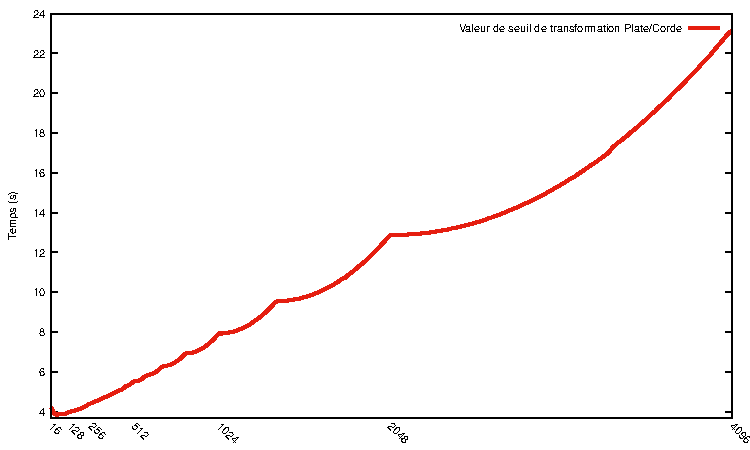
\includegraphics[]{figures/index_maxlen.pdf}
\end{figure}

Nous observons dans ce cas que la meilleure valeur de seuil, produisant des résultats minimaux est 64.
Moins que cela, le temps de parcours de la corde devient le facteur limitant, et plus que cela, le temps augmente du
fait du parcours de la chaîne plate en temps linéaire.

Les résultats sont disponibles via le tableau~\ref{index_maxlen_dat} et la figure~\ref{index_maxlen_fig}.

\subsection{Itération}

Dans ce benchmark, nous effectuons 200k itérations sur une chaîne construite procédura-lement via
des concaténations successives en début d'exécution.

\begin{table}
	\caption{\label{iter_maxlen_dat}Temps en secondes pour 200k itérations sur une chaîne de longueur 4096, en fonction du seuil de transformation corde/plate.}
	\centering
	$\begin{array}{ *{10}{c} }
		\toprule
		& 16 & 32 & 64 & 128 & 256 & 512 & 1024 & 2048 & 4096 \\
		\midrule
		& 7.47 & 6.42 & 5.91 & 5.67 & 5.55 & 5.48 & 5.47 & 5.46 & 5.3\\
		\bottomrule
	\end{array}$
\end{table}

\begin{figure}
	\caption{Temps en secondes pour 200k itérations en fonction de la longueur de la chaîne, par variation de seuil de transformation corde/plate.}
	\label{iter_maxlen_fig}
	\centering
	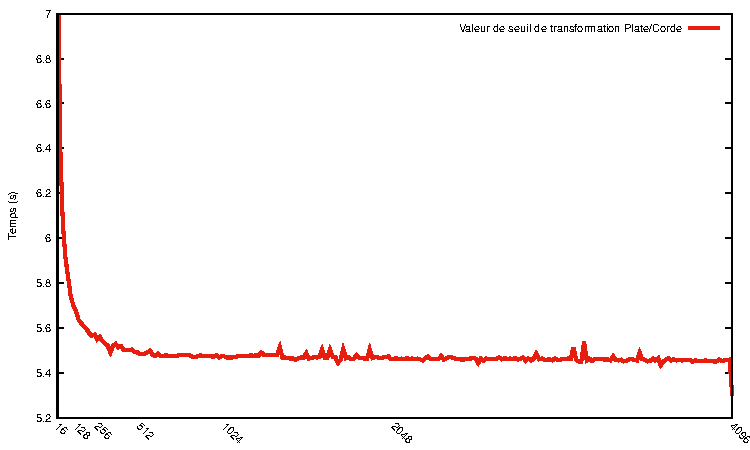
\includegraphics[]{figures/iteration_maxlen.pdf}
\end{figure}

Sans surprise ici, plus la chaîne est plate, plus l'itération est rapide, l'opération ne nécessitant pas de parcourir
de corde.
Cependant, la différence commence à être moindre à partir de 512 octets par feuille.
On notera que dans ce cas, la baisse à 4096 est due au manque total de cordes, ce qui induit un nombre plus faible d'indirections et donc une meilleure performance.

Les résultats sont disponibles via le tableau~\ref{iter_maxlen_dat} et la figure~\ref{iter_maxlen_fig}.

\subsection{Sous-chaînage}

Dans ce benchmark, nous effectuons 5M sous-chaînages successifs avec des bornes aléa-toires sur une chaîne construite
procéduralement via des concaténations successives en début d'exécution.

\begin{table}
	\caption{\label{substr_maxlen_dat}Temps en secondes pour 5M sous-chaînages en fonction de la longueur de la chaîne, par variation de seuil de transformation corde/plate.}
	\centering
	$\begin{array}{ *{10}{c} }
		\toprule
		& 16 & 32 & 64 & 128 & 256 & 512 & 1024 & 2048 & 4096\\
		\midrule
		& 38.81 & 20.06 & 10.16 & 5.40 & 3.29 & 2.06 & 1.95 & 2.49 & 3.35\\
		\bottomrule
	\end{array}$
\end{table}

\begin{figure}
	\caption{Temps en secondes pour 5M sous-chaînages en fonction de la longueur de la chaîne, par variation de seuil de transformation corde/plate.}
	\label{substr_maxlen_fig}
	\centering
	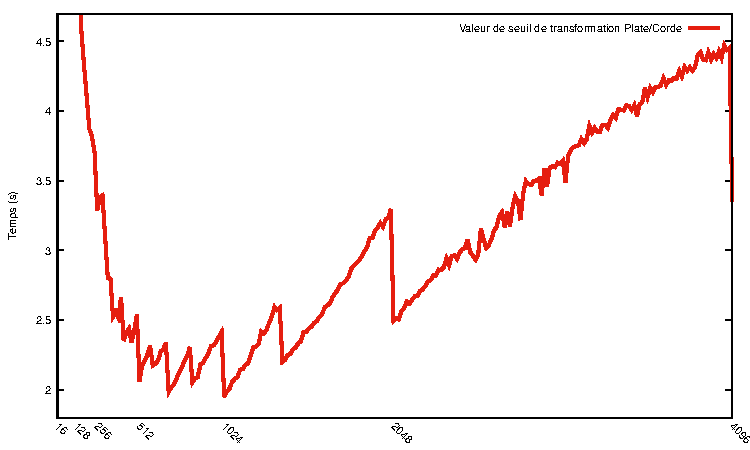
\includegraphics[]{figures/substring_maxlen.pdf}
\end{figure}

Les résultats obtenus en~\ref{substr_maxlen_dat} nous offrent des résultats intéressants,
comme le montre la figure~\ref{substr_maxlen_fig}.
En effet, le temps total de sous-chaînage dans ce cas va dépendre de la taille de seuil
de façon importante.
Une valeur de seuil trop faible entraîne le plus de surcoût dans notre cas, principalement
du a la reconstruction des noeuds de corde que produit cette approche.
Cette reconstruction entraîne la création de beaucoup d'objets éphémères, ce qui
a pour effet d'augmenter la pression sur le ramasse-miettes, et par ce fait, le
temps d'exécution augmente autant.
Cette mesure exclut le temps de ré-équilibrage des cordes, qui ferait encore augmenter
les temps d'exécution dans ce cas-ci.
On notera également qu'à partir d'une valeur de seuil de 1024, le temps recommence à
augmenter, cette fois-ci à cause du temps de parcours des feuilles, ce dernier augmentant linéairement.
Dans ce cas-ci, les meilleures valeurs de seuils à considérer sont donc comprises entre
512 et 1024.

\subsection{Conclusion}

Dans ces benchmarks, nous remarquons que dans une majorité de cas, des longueurs de feuille
aux alentours de 512 ou 1024 semblent apporter le meilleur compromis.
Cela nous conforte dans notre choix d'utiliser 512 dans notre implémentation comme seuil de passage
de chaîne plate vers corde.

\section{Étude de cas: Lecture de JSON}\label{json_perf}

JSON (JavaScript Object Notation) est un format de représentation de données
sous forme de chaînes de caractères.
Il est défini dans la RFC 7159 \cite{bray2014javascript} comme le format d'échange de
données par défaut pour le langage Javascript.
Il permet la représentation hiérarchique des données sous forme d'objets, sa grammaire
est simple et ne nécessite que peu de métadonnees pour représenter de l'information,
ce qui en fait un format efficace.
Depuis son introduction, il est devenu, à la date de redaction de ce document, l'un
des formats les plus populaires pour l'échange de données via Internet\cite{wang2011improving}.

De par son statut hégémonique, une majorité de langages de programmations populaires
modernes possèdent une implémentation d'analyseur syntaxique de JSON dans leur bibliothèque
standard. C'est le cas de Python, Ruby, Go, etc.

Cette sous-section identifie et compare les implémentations de plusieurs analyseurs syntaxiques
JSON dans differents langages: C, Go, Ruby, Python 2, Python 3 et Nit.
Deux alternatives sont présentées pour Nit: un analyseur syntaxique géneré par un outil, et un analyseur
syntaxique écrit à la main.

\subsection{Implémentations}

Les implémentations d'analyseurs syntaxiques JSON que nous étudions sont comparables au niveau de la
fonctionnalité, chacun est capable de lire une chaîne de caractères en JSON valide et de la
transformer en un objet natif du langage pour permettre son utilisation par la suite.
Les erreurs de formattage sont repérées, et renvoyées à l'utilisateur.

Les principales différences entre les implémentations viennent majoritairement de la
technique d'implémentation, du niveau d'optimisation et de la gestion du codage.

Ruby expose deux versions d'analyseur syntaxique JSON: l'une implementée en Ruby pur, qui est laissée
en dehors des chiffres du fait de sa lenteur et une autre utilisant un automate déterministe
à états finis optimisé généré en C\footnote{
\url{https://github.com/ruby/ruby/tree/c4fdfabcc8ea3f6186d1560f7756211fce125be3/ext/json/parser}.}
directement par un outil externe: Ragel \cite{ragel}.

Python possède également deux versions d'analyseur syntaxique JSON dans sa bibliotheque standard,
toutes deux implementées dans l'engin de référence du langage, \texttt{cpython}.
L'une est implémentée de facon efficace en C\footnote{\url{https://github.com/python/cpython/blob/master/Modules/_json.c}.}.
La seconde est en Python pur\footnote{\url{https://github.com/python/cpython/blob/master/Lib/json/decoder.py}.},
et sera automatiquement utilisée en cas de non-disponibilité de l'analyseur syntaxique C.
Notons que dans le cas de Python, nous faisons une différence entre la version 2 et la version
3 du langage et de l'engin d'éxécution à cause notamment de la différence de manipulation
des chaînes de caractères entre les deux versions \cite{PEP393}.

C n'a pas d'analyseur syntaxique JSON de référence, essentiellement car la bibliothèque standard
de C est assez primitive, les fonctionnalités sont souvent ajoutées via des surcouches externes.
Nous prendrons ici comme référence l'analyseur syntaxique \texttt{ujson4c}\footnote{Disponible ici \url{https://github.com/esnme/ujson4c}.}.

Go quant à lui offre un analyseur syntaxique JSON écrit complètement à la main et disponible
dans sa bibliothèque standard\footnote{\url{https://golang.org/src/encoding/json/decode.go}.}.

Pour finir, Nit expose deux implémentations d'analyseurs syntaxiques JSON.
L'un généré par NitCC\footnote{NitCC est un générateur d'analyseurs lexicaux et syntaxiques à partir d'un fichier de grammaire.},
qui produit un ensemble d'analyseurs lexicaux et syntaxiques complet pour la grammaire
de JSON. Il produit un AST\footnote{Abstract Syntax Tree, un arbre organisant hiérarchiquement les
entités d'un texte.} intermédiaire lors du parsing, ce qui en fait un analyseur syntaxique inefficace.
À cause de cela, il est mentionné, mais pas inclus dans les résultats.
Un deuxième analyseur syntaxique est une implémentation de machine à états finis en Nit pur.
Deux programmes clients de cet analyseur syntaxique sont mis à l'épreuve: l'un utilisant un mélange de cordes et
de chaînes plates, et un deuxième comptant seulement des chaînes plates.
Tous prennent en compte Unicode dans leurs routines de chaînes de caractères.

\subsection{Protocole d'expérimentation}

Les analyseurs syntaxiques sont chacun lancés sur des fichiers d'une longueur variable et avec des contenus plus ou
moins complexes.
Chaque fichier de la suite est codé en UTF-8.

\begin{enumerate}
	\item Un premier fichier\footnote{Disponible via \url{https://edg.epa.gov/data.json}.} de 6.6 Mio contenant du texte ASCII, copié 10 fois dans un tableau JSON pour un fichier de 66 Mio au total - Gov
	\item Un deuxième fichier\footnote{Disponible via \url{https://raw.githubusercontent.com/miloyip/nativejson-benchmark/master/data/twitter.json}.} de 65 kio contenant des caractères japonais, copié 200 fois dans un tableau JSON, pour un fichier de 60 Mio au total - Twitter
	\item Un troisième fichier\footnote{Disponible via \url{https://github.com/seductiveapps/largeJSON/blob/master/100mb.json?raw=true}.} de 100 Mio contenant beaucoup de caractères echappés sous la forme \textbackslash uXXXX - Large
	\item Un dernier fichier\footnote{Disponible via \url{http://mtgjson.com/json/AllSets-x.json}.} de 40 Mio contenant des caractères Unicode et ASCII - Magic
\end{enumerate}

Chaque analyseur syntaxique lit et analyse l'entrée pour créer des objets natifs au langage cible.
Chaque benchmark est exécuté 5 fois sur le fichier, et la moyenne du temps est retenue comme donnée de base, les
temps minimum et maximum sont gardés et représentés dans le graphique final.

\subsection{Résultats et discussion}

Parmi les analyseurs syntaxiques étudiés, sans surprise, la bibliotheque C \texttt{ujson4c} est la plus efficace.
En s'affranchissant de la sémantique d'Unicode quant à l'accès à un caractère et en effectuant des comparaisons
efficaces lors de la recherche d'échappements (switchs, accès à des tables pré-calculées), il est entre 4 et 5
fois plus rapide que l'implémentation Python 3.

Python 3 est la deuxième implémentation en termes d'efficacité, suivie par Python 2.
Le fait que l'analyseur syntaxique soit écrit directement en C est une aide significative dans ce cas-ci.
Notons que la différence entre Python 2 et Python 3 vient majoritairement de l'introduction de PEP-393, Python
2 perdant effectivement une partie du temps alloué à la transformation de la chaîne entrée en chaîne Unicode
Python.

\begin{table}
	\caption{\label{JSON_parse_time}Temps de parsing de fichiers JSON en fonction du langage}
	\centering
	$\begin{array}{ *{8}{c} }
		\toprule
		 & C & Python 3 & Python 2 & Go & Nit - Cordes & Nit + Cordes & Ruby \\
		\midrule
		Gov & 0.11 & 0.55 & 1.00 & 1.15 & 1.14 & 1.30 & 1.33\\
		Twitter & 0.11 & 0.7 & 1.10 & 1.12 & 1.14 & 1.24 & 1.29\\
		Large & 0.27 & 1.23 & 1.7 & 2.96 & 3.25 & 3.44 & 3.75\\
		Magic & 0.13 & 0.87 & 1.58 & 1.40 & 1.37 & 1.45 & 2.94\\
		\bottomrule
	\end{array}$
\end{table}

\begin{figure}
	\caption{Parsing JSON par langage}
	\label{jsonparse}
	\centering
	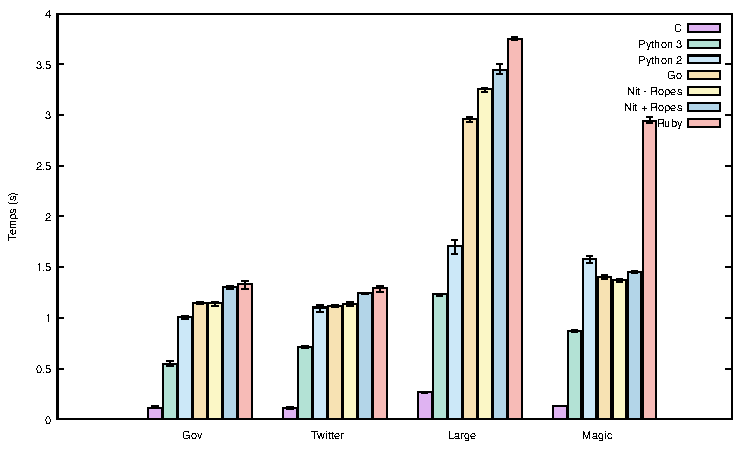
\includegraphics[]{figures/parse_json.pdf}
\end{figure}

Go est 4$^{e}$ en termes d'efficacité avec son implémentation native d'analyseur syntaxique JSON.
L'implementation Nit occupe la place qui suit, avec des résultats proches de Go. Les résultats sont
cohérents du fait de la similarité des implémentations.
En Nit, la majorité du temps est passée dans les routines de décodage de chaînes de caractères qui,
à cause d'UTF-8, augmentent le temps passé dans les accès indexés.
Un ralentissement est observé en Nit dans la version utilisant des cordes (identifiée dans le tableau~\ref{JSON_parse_time}
comme \texttt{Nit + Cordes}), cela s'explique par les performances
réduites des cordes en itération et sous-chaînage, dans un cadre où le programme les utilise intensivement, mais où
peu, voire aucune concaténation, ni accès indexé aléatoire ne sont effectués.
On notera cependant que le ralentissement observé reste du domaine de l'acceptable dans la mesure où il reste sous les
8\%, à l'exception de Gov, où il approche 15\% de différence.
Nous attribuons ce changement au fait que Gov est un fichier JSON entièrement en ASCII, sans caractères échappés,
ce qui permet aux optimisations des chaînes plates dans ce cas particulier de briller.
Ruby est en dernière place de ce comparatif, et ce malgré son implémentation C efficace.

La version NitCC, qui n'a pas été retenue pour ce comparatif, est plus lente que
la version Ruby avec un analyseur syntaxique C.
Son temps pour le fichier \texttt{Gov} est de 3.957 s, plus lente d'un facteur superieur à
2 par rapport à la version Ruby/C.
Le temps de l'analyseur syntaxique Ruby en version ruby-pure est, pour le même fichier de 7.805 s, soit près de 6 fois plus
lente que son équivalent optimisé.

\section{Étude de cas: Analyse syntaxique de documents CSV}

CSV, à l'instar de JSON, est un format de stockage de données textuelles sous forme de table.
Il est par exemple utilisé pour stocker de façon portable des données issues de tableurs comme
Microsoft Excel ou Libre Office Calc entre autres.

Il s'agit d'un format ancien, pas nécessairement en tant que fichier de données, mais comme représentation
simple de données, tel que représenté en IBM Fortran \cite{ibmfortran74} via les \texttt{FORMAT statements}.
Depuis, le format a été utilisé par un nombre conséquent de programmes et utilisateurs pour
échanger des données.
Une tentative de normalisation a été effectuée en 2005 par le biais de la RFC 4180 \cite{rfccsv}.
Cette dernière se base sur les trois principes suivants:

\begin{enumerate}
	\item Les séparateurs sont définis comme le caractère virgule (,)
	\item Les fin de lignes sont signalées par la séquence de caractères CRLF (\textbackslash r \textbackslash n)
	\item Les séquences contenant soit un séparateur, soit une fin de ligne, soit un caractère d'échappement, doivent être échappées via un caractère d'échappement ("). Ceux-ci sont doublés lorsque présents dans la chaîne échappée.
\end{enumerate}

Cette section vise à comparer plusieurs implémentations d'analyseurs syntaxiques CSV dans plusieurs langages,
sur de larges fichiers CSV.
Nous allons comparer ici les implémentations de la bibliothèque standard de Python, Ruby, Nit et Go.
Nous allons également comparer l'implémentation Java d'Apache, via le package Apache Commons
\footnote{Disponible à \url{http://apache.mirror.gtcomm.net//commons/csv/binaries/commons-csv-1.3-bin.zip}}, dans sa version 1.3.
En ce qui concerne Python, nous allons également mesurer la performance de l'analyseur de la bibliothèque
Pandas, basée sur NumPy.

\subsection{Implémentations}

A l'instar du protocole de test pour JSON, toutes les bibliothèques que nous comparons offrent des
fonctionnalités similaires.
Chaque bibliothèque aura pour but lors du test de lire un fichier CSV et de le transformer en une structure
tabulaire utilisable dans un programme écrit dans le langage cible.

Des différences seront à noter en ce qui concerne l'API de certains cependant. Python - Pandas, Nit, Go et Ruby
fonctionnent via une approche globale.
C'est à dire qu'a partir d'un fichier ou d'une chaîne de caractère, ils sont
capables de produire un tableau contenant l'ensemble des données du document en un seul appel de fonction.
Les approches suvies par Java - Apache Commons et Python - Standard, sont elles orientées sur un mécanisme
d'itérateur.
Il est donc nécessaire dans leur cas de lire le document ligne par ligne pour en stocker son contenu dans une
table.
Cette opération possède le désavantage de produire plus d'appels de fonctions, possiblement polymorphes,
ce qui induit nécessairement un ralentissement par rapport à une approche globale.

\subsection{Protocole d'expérimentation}

Chaque analyseur syntaxique sera lancé sur des fichiers contenant 1 million de lignes, plus une
ligne d'entête.
Deux fichiers générés via un outil écrit en Nit seront considérés pour cette étude:

\begin{enumerate}
	\item \texttt{1M lignes ASCII}: Un fichier contenant 1 million de lignes de données, chacune contenant 10 éléments d'une longueur aléatoire comprise entre 1 et 15 caractères \texttt{a} ainsi que des caractères nécessitant l'échappement de façon aléatoire.
	\item \texttt{1M lignes UTF-8}: Un fichier contenant 1 million de lignes de données, chacune contenant 10 éléments d'une longueur aléatoire comprise entre 1 et 15 caractères \texttt{à} ainsi que des caractères nécessitant l'échappement de façon aléatoire.
\end{enumerate}

Chaque benchmark est exécuté 5 fois sur le fichier, la moyenne du temps utilisateur est retenue comme donnée de base.
Les temps minimum et maximum sont égalements gardés pour mesurer la variabilité du test.

\subsection{Résultats et discussion}

\begin{table}
	\caption{\label{csv_numbers}Temps de parsing de fichiers CSV en fonction du langage}
	\centering
	$\begin{array}{ *{10}{c} }
		\toprule
		& \rotatebox[]{65}{Ruby} & \rotatebox[]{65}{Java} & \rotatebox[]{65}{Go} & \rotatebox[]{65}{Python2} & \rotatebox[]{65}{Python3} & \rotatebox[]{65}{Nit-Cordes} & \rotatebox[]{65}{Nit+Cordes} & \rotatebox[]{65}{Pandas2} & \rotatebox[]{65}{Pandas3}\\
		\midrule
		ASCII & 67.33 & 10.28 & 3.02 & 2.77 & 3.38 & 1.59 & 1.92 & 1.08 & 1.11\\
		Unicode & 70.15 & 10.59 & 3.79 & 2.96 & 3.67 & 3.24 & 3.65 & 1.25 & 1.3\\
		\bottomrule
	\end{array}$
\end{table}


Parmi les analyseurs étudiés, Python - Pandas est le plus efficace.
Sa rapidité vient du fait que la bibliothèque est principalement écrite en C et optimisée autant
que possible.
Les sémantiques d'accès aux caractères imposées par Unicode ne s'appliquent pas à leur analyseur, et la majorité
du code étant écrite et compilée avec les fanions d'optimisation maximum font de lui le plus rapide.

Ensuite, nous avons l'implémentation Nit, un parseur écrit à la main en Nit pur.
L'analyseur respecte les sémantiques d'Unicode pour l'accès aux caractères et les manipulations sur le contenu
d'une chaîne.
Un effort particulier a été apporté pour assurer une performance optimale dans le cas d'une bibliothèque écrite
en Nit pur.
La version utilisant les cordes est, à l'instar de l'analyseur JSON, plus lente que la version ne les utilisant pas,
dans une marge acceptable (entre 5 et 10\%).
On notera que le fichier contenant des chaînes Unicode est beaucoup plus lente que celle contenant des chaînes uniquement
ASCII.
Cette différence s'explique du fait des optimisations effectuées dans la bibliothèque du langage pour accélérer le traitement
des chaînes ASCII, statistiquement plus fréquentes.

Les implémentations Go et Python - Standard offrent une performance similaire, les deux étant écrits dans des langages
proches de la machine pour en améliorer la performance.
On notera cependant que Python 2 est légèrement plus rapide que Python 3 dans ce cas-ci, ce dernier s'affranchissant
des préoccupations d'Unicode et ne nécessitant pas de travail préalable pour la construction d'une chaîne de caractères.
Dans ce cas particulier, PEP-393 provoque un ralentissement de l'implémentation Python.

Java est avant dernier dans ce test, avec un temps près de 3 fois plus lent que les implémentations Go et
Python - Standard.
On notera que dans le cas de Java, le fichier comportant de l'Unicode ne provoque pas de ralentissement lors
de la phase d'analyse.
Ce comportement s'explique du fait de l'étape de conversion du contenu du fichier vers UTF-16.
Une fois la conversion effectuée, la lecture des caractères s'effectue en temps constant dans ce cas.

Ruby, avec une implémentation en pur Ruby, est la plus lente de notre comparatif, près de 7 fois plus
lente que l'implémentation Java.

L'ensemble des résultats sont disponibles via le tableau \ref{csv_numbers} et la figure \ref{csv_graph}.

\begin{figure}
	\caption{Parsing CSV par langage}
	\label{csv_graph}
	\centering
	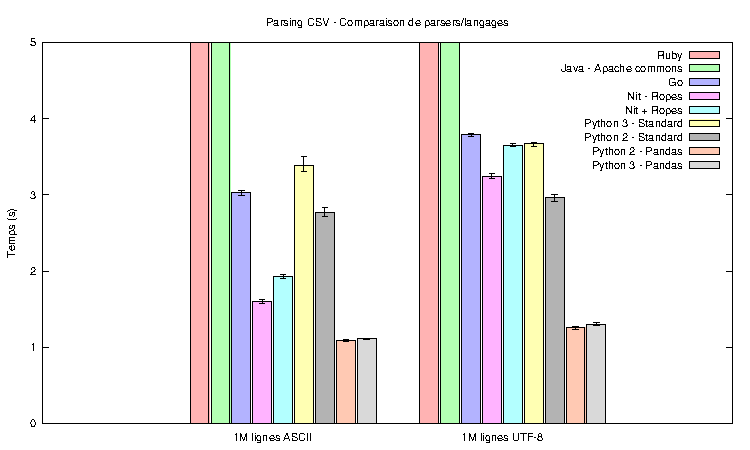
\includegraphics[]{figures/csv_bench.pdf}
\end{figure}

\section{Étude de cas: Le compilateur Nit, nitc}

Le compilateur est un des programmes les plus importants de la base de code de Nit.
Puisqu'il s'agit d'un programme indispensable à tout développeur Nit, il se doit
d'être le plus performant possible.
Dans la mesure où une grande partie de son travail consiste à lire, traiter et générer
du texte, il s'agit d'un cas très pertinent pour cette étude.

Nous allons uniquement comparer des variations de techniques de gestion des chaînes
de caractères et exposer le temps moyen d'exécution sur 5 exécutions du compilateur
se compilant lui-même.
Afin d'assurer plus de stabilité dans les chiffres et de minimiser l'impact de la
compilation du C généré par `nitc`, nous allons pré-compiler 4 fois le compilateur
avec lui-même avant d'effectuer la mesure.

Nous allons étudier l'impact sur deux techniques de compilation de nitc, en compilation
séparée et en compilation semi-globale.
Cette dernière effectuant plus d'optimisations en supposant une connaissance globale
du programme compilé; elle effectuera plus
d'\texttt{inlining}\footnote{Extension d'une méthode directement dans le code généré, évitant le coût de l'appel.}
de méthodes et remplacera
certains appels polymorphes par des appels monomorphes, resultant en un code globalement
plus efficace.

\subsection{Résultats et discussion}

Le tableau \ref{nitc_time} et les figures \ref{nitc_sep} et \ref{nitc_sg_vars} présentent les résultats de
la compilation de nitc avec nitc, en compilation séparée et semi-globale.
Comme attendu, la version semi-globale est plus rapide que la version
séparée.

\begin{table}
	\caption{\label{nitc_time}Temps d'exécution de `nitc src/nitc.nit` en fonction des variations d'implémentation de chaînes de caractères}
	\centering
	$\begin{array}{ *{6}{c} }
		\toprule
		 & Cordes + Plates & Plates & Cordes & Lineaire & Buffered \\
		\midrule
		separate & 3.9 & 4.11 & 4.33 & 3.86 & 4.10\\
		semi-global & 3.75 & 3.95 & 4.13 & 3.73 & 4.06\\
		\bottomrule
	\end{array}$
\end{table}

\begin{figure}
	\caption{Temps d'exécution de la commande `nitc src/nitc.nit --separate` en fonction des variations d'implémentation de chaînes de caractères}
	\label{nitc_sep}
	\centering
	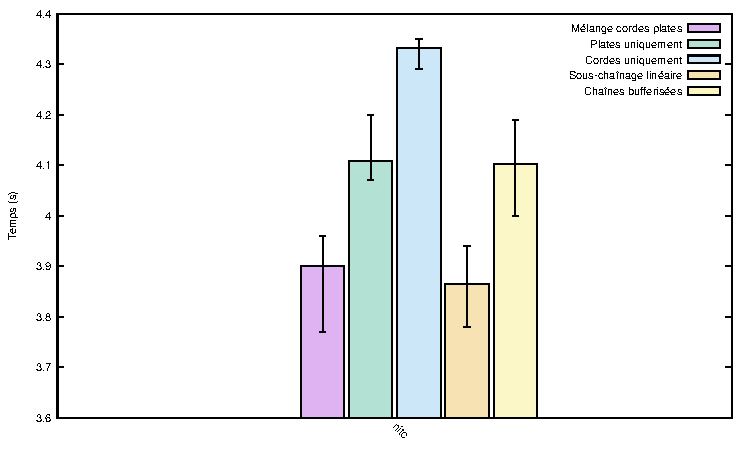
\includegraphics[]{figures/nitc_separate_vars.pdf}
\end{figure}

\begin{figure}
	\caption{Temps d'exécution de la commande `nitc src/nitc.nit --semi-global` en fonction des variations d'implémentation de chaînes de caractères}
	\label{nitc_sg_vars}
	\centering
	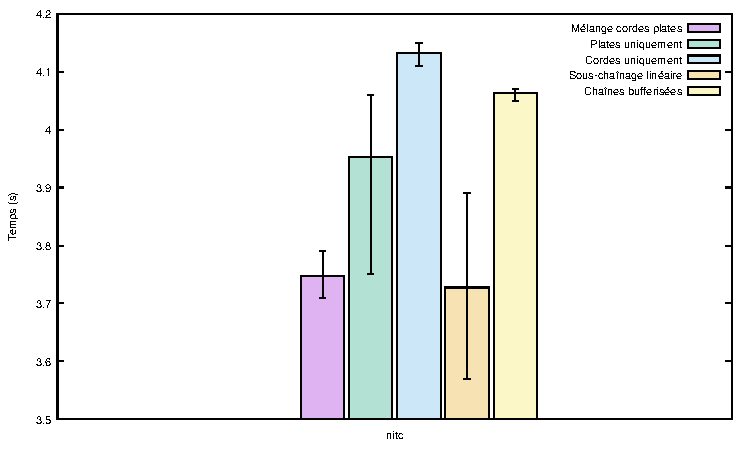
\includegraphics[]{figures/nitc_semi-global_vars.pdf}
\end{figure}

La version de base, celle qui est présentement implémentée et utilisée dans la bibliothèque
standard de Nit est la version utilisant le mélange de cordes et de chaînes plates.

Parmi les variations étudiées, nous remarquons que la variation utilisant une opération de
sous-chaînage en temps linéaire est plus rapide que ses équivalentes utilisant le partage
de chaînes.
Nous attribuons cet avantage à la structure plus légère de la chaîne produite, ce qui permet
à l'ensemble des opérations subséquentes de s'effectuer plus rapidement.
Le surcoût induit par la réallocation et la copie de la chaîne est moindre comparé
aux bénéfices de temps sur le reste des opérations.

Les chaînes sur-allouantes ne présentent pas de véritable gain dans cette configuration et font
perdre du temps, cette perte peut être imputée en grande partie aux indirections supplémentaires
et à l'alourdissement de la structure.
Dans le cas du compilateur, il est à noter également que les concaténations multiples sont rares,
car optimisées à l'aide de \texttt{Buffers}.
Il est donc normal dans ce cas de figure que la solution n'apporte pas de réel bénéfice.
Il s'agit cependant du cas le plus fréquent dans les applications optimisées pour ce genre
d'utilisations.

Les cordes systématiques sont peu pertinentes dans la mesure où les concaténations sont
réalisées via des buffers dans une majorité de cas, mais où les accès et itérations sont
fréquents, ce qui a pour conséquence de ralentir l'exécution.

Les chaînes uniquement plates sont elles aussi perdantes dans ce cas de figure, le principal
défaut de cette approche étant que le travail de parcours de chaîne est onéreux lorsqu'effectué
loin du cache.
Ce cas-ci est rare, mais présent dans le compilateur lors de la production tardive d'une sous-chaîne
pour récupérer le contenu d'un jeton lors de phases d'analyses subséquentes.
La limite de la taille des feuilles et l'accès en O(log(n)) sont ici bénéfiques.

\subsection{Variation du seuil de concaténation}

Nous incluons le compilateur dans nos benchmarks de vérification du seuil par défaut des transformations
de chaines plates vers cordes.
Le modus operandi ici est similaire à celui utilisé dans les micro-benchmarks en \ref{rope_flat_thres_bench},
en faisant varier le seuil de transformation sur des puissances de 2, de 16 à 4096.

\begin{table}
	\caption{\label{nitc_time_maxlen}Temps d'exécution de `nitc src/nitc.nit` en fonction du seuil de conversion plate/corde}
	\centering
	$\begin{array}{ *{10}{c} }
		\toprule
		& 16 & 32 & 64 & 128 & 256 & 512 & 1024 & 2048 & 4096 \\
		\midrule
		separate & 4.23 & 3.93 & 3.94 & 3.88 & 3.91 & 3.95 & 3.95 & 3.9 & 3.93\\
		semi-global & 4.05 & 3.72 & 3.77 & 3.75 & 3.70 & 3.74 & 3.73 & 3.72 & 3.76\\
		\bottomrule
	\end{array}$
\end{table}

\begin{figure}
	\caption{Temps d'exécution de la commande `nitc src/nitc.nit` en fonction du seuil de conversion plate/corde}
	\label{nitc_sep_maxlen}
	\centering
	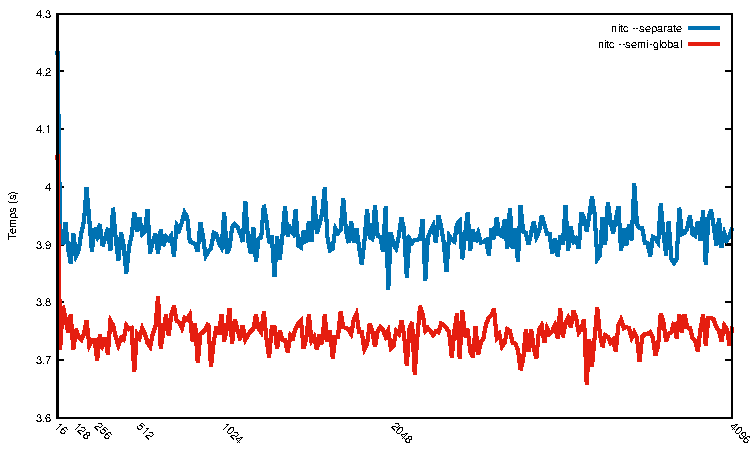
\includegraphics[]{figures/nitc_separate_maxlen.pdf}
\end{figure}

Nous observons cependant peu de différences dépendamment directement du seuil, pourvu que celui-ci
soit au moins de 32.
Les résultats sont disponibles via le tableau~\ref{nitc_time_maxlen} et la figure~\ref{nitc_sep_maxlen}.

\section{Étude de cas: nitlight}

Nitlight est un outil écrit en Nit base sur la chaîne d'outils dérivée du
compilateur.
Il sert à produire des fichiers HTML contenant le code source d'un fichier
coloré, avec des liens sémantiques vers la documentation et les entités
comprises dans le code.

Par sa nature d'analyseur et producteur de chaînes, ce dernier est intéressant
pour juger de la performance de notre implémentation, et plus particulièrement
pour étudier les différents seuils de transformation de chaîne plate vers corde.

Ce benchmark va lancer nitlight pour compiler les fichiers HTML liés au compilateur
ainsi que toutes ses dépendances.
Le modus operandi pour la mesure de la performance est identique à celui
utilisé précédemment.

\subsection{Résultats et discussion}

Comme dans le cas du compilateur, la variation du seuil de transformation
ne s'avère pas avoir beaucoup d'effet passé un seuil minimal de 64.
En effet, passé ce seuil, la durée d'une exécution reste stable, avec une variation de +/- 0.1s.

\begin{table}
	\caption{\label{nitlight_time_maxlen}Temps d'exécution de `nitlight --full -d out\_dir nitc.nit` en fonction du seuil de conversion plate/corde}
	\centering
	$\begin{array}{ *{10}{c} }
		\toprule
		& 16 & 32 & 64 & 128 & 256 & 512 & 1024 & 2048 & 4096\\
		\midrule
		separate & 6.45 & 6.42 & 5.91 & 5.86 & 5.83 & 5.97 & 5.94 & 5.98 & 5.83\\
		semi-global & 5.74 & 5.70 & 5.37 & 5.31 & 5.32 & 5.37 & 5.31 & 5.32 & 5.35\\
		\bottomrule
	\end{array}$
\end{table}

\begin{figure}
	\caption{Temps d'exécution de la commande `nitlight --full -d out\_dir nitc.nit` en fonction du seuil de conversion plate/corde}
	\label{nitlight_sep_maxlen}
	\centering
	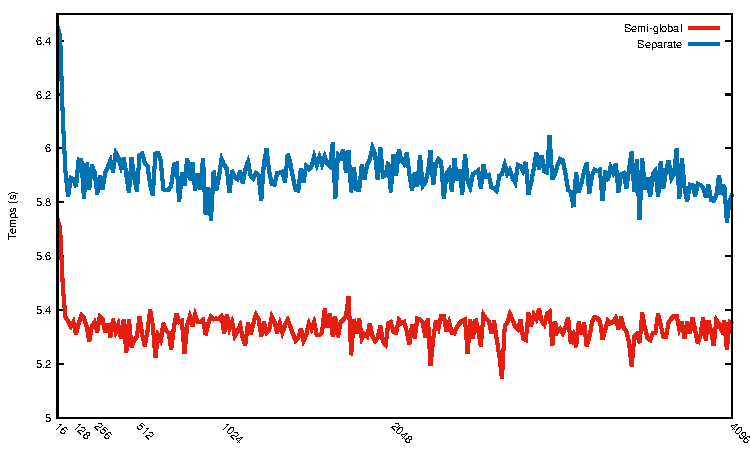
\includegraphics[]{figures/nitlight.pdf}
\end{figure}

Les résultats sont disponibles via le tableau~\ref{nitlight_time_maxlen} et la figure~\ref{nitlight_sep_maxlen}.

\section{Conclusion}

Ce chapitre présente une suite de programmes de mesure de la performance, constituant une validation de notre solution.
En effet, en mélangeant les cordes aux chaînes plates, et en utilisant une stratégie efficace pour la production de ces
dernières, nous mitigeons les cas dégénératifs exposés par les deux structures, et pouvons utiliser l'une représentation
ou l'autre de façon complètement transparente.

Des optimisations restent cependant à étudier pour limiter encore les problèmes que posent une
structure arborescente pour les chaînes dans les cas courants, tels que nous pouvons voir dans 
l'analyseur syntaxique JSON.


% Utilisez l'environnement  conclusion pour rédiger votre conclusion
\begin{conclusion}

Dans cette étude, nous traitons des implémentations des chaînes de caractères dans les langages de programmation et des problématiques de performance qui en découlent.
Nous avons identifié les cas dégénératifs d'utilisation des chaines plates:

\begin{enumerate}
	\item concaténation: la ré-allocation et la copie sur de grandes chaînes;
	\item accès indexé: dû aux codages à longueur variable, l'opération est en O(n);
	\item modification: pour les mêmes raisons que l'accès indexé, le déplacement jusqu'à la position à modifier, et
		la modification, qui peut entraîner le déplacement d'une partie de la chaîne.
\end{enumerate}

Pour chaque problème des chaînes plates, les cordes sont une réponse appropriée.
Cependant, elles aussi exposent des cas dégénératifs:

\begin{enumerate}
	\item sous-chaînage: le parcours et la création des nouveaux noeuds de la corde peuvent empêcher à l'opération de s'effectuer en un temps raisonnable;
	\item itération: le parcours de la corde ralentit l'opération.
\end{enumerate}

Nous avons décidé de mélanger les deux approches dans une solution originale afin de profiter des avantages des
deux structures, et de mitiger leurs inconvénients.
Nous avons implémenté cette solution dans le langage Nit, et la transition d'une structure à l'autre s'effectue
de façon transparente pour l'utilisateur lors d'une concaténation via un système de seuil de conversion.

La question du codage des caractères est également traitée lors de cette étude.
En 2016, tous les langages de programmation se doivent de supporter au moins un des codages prévus et spécifiés
par Unicode, que ce soit par défaut (Nit, Go, Python, Ruby, etc.) ou par le biais de bibliothèques (C, C++, etc.).
Ces choix ont cependant des conséquences en termes de performance ou d'utilisation mémoire.

Nous avons choisi en Nit d'utiliser UTF-8 par défaut, ce choix a été motivé par les facteurs de popularité
du codage et de compatiblitité avec les chaînes C.
Ces deux avantages nous garantissent de pouvoir continuer à utiliser des fonctions de manipulations de chaînes
de caractères implémentées en C pour des raisons de performance, mais également de limiter la probabilité
d'avoir un travail de conversion à effectuer lors de la lecture de texte.
UTF-8 est également le codage Unicode le plus économe en termes de mémoire\footnote{À l'exception du rare cas
de texte contenant uniquement des caractères asiatiques, où UTF-16 est plus économe.}, ce qui garantit
une consommation raisonnable.

Nous apportons un modèle de représentation original de chaînes de caractères, efficace et simple à utiliser.
Il garantit:
\begin{enumerate}
	\item La non-dégénérescence des opérations effectuées sur les chaînes de caractères
	\item Une meilleure gestion de la mémoire en limitant l'espace contigu nécessaire pour stocker une chaîne entière
	\item De meilleures performances de ramasse-miettes en évitant d'allouer des blocs de
		texte trop grands et en évitant de copier ou déplacer des données d'un endroit à l'autre de
		la mémoire lors de manipulations de chaînes de caractères.
\end{enumerate}

La solution que nous présentons est viable, comme le montrent les résultats que nous présentons dans le
chapitre~\ref{perf_chap} sur la performance, aussi bien sur de micro-benchmarks que sur des programmes réels.
En effet, cette solution limite les effets des cas dégénératifs dans tous les cas.
Cependant, son impact sur des programmes réels est variable.
Notons que si une accélération n'est pas toujours constatée, la performance reste égale ou tout du moins
proche par rapport à une approche utilisant uniquement des chaînes plates.
Elle accuse par exemple un ralentissement moyen de 8\% sur le cas d'analyse syntaxique JSON, un cas
défavorable à l'utilisation des cordes.

Dans le futur, la bibliothèque continuera à évoluer, de façon à améliorer ses performances
dans les cas présentés.
Nous continuons activement la recherche de meilleures heuristiques pour la production de cordes
dans des cas d'utilisation courants.

En termes de codage, il reste à explorer la possibilité de transiter vers une API orientée graphème,
à l'instar des implémentations de Swift et Perl6.
Cette modification aurait pour conséquence d'alourdir la représentation de caractère, n'étant plus
primitive.

Il est cependant possible d'imaginer une solution transformant \texttt{Char} en une structure abstraite
et en implémentant les différents cas: graphème simple (point de code), graphème étendu, etc.
À l'implémentation de cette solution, il faudra évaluer l'impact sur la performance, le passage
d'un type primitif à un type abstrait empêchant les optimisations à la génération du code (inlining
impossible, nécessité d'utiliser des appels polymorphes pour les fonctions de \texttt{Char}, etc.).

Le développement et l'optimisation de la version mutable de notre solution restent également à repenser
afin de réduire les problèmes inhérents aux codages à longueur variable dans les cas de modification et d'avoir
des performances proches des \texttt{buffers} actuels dans le cas de la concaténation.

Il reste encore également des possibilités d'évolution sur l'architecture elle-même.
Il est possible pour le sous-chainage par exemple, de proposer une implémentation adaptative, ré-allouant
et copiant les données sous un seuil, et partageant les sous-chaînes dans d'autres cas.

Une autre possibilité pour améliorer les performances est de se baser sur des techniques d'analyse de code
pour changer les représentations à la compilation ou ajouter des optimisations dans des cas limites.
\end{conclusion}


%%%%%%%%%%%%%%%%%%%%
% Page liminaires
%%%%%%%%%%%%%%%%%%%%
\bibliographystyle{theseuqam2} % non compatible avec le package natbib
\bibliography{bibliography}

\end{document}
